\section{Introduction}

In this chapter I examine whether adding feedback loops to the genetic toggle switch increases its parametric robustness to parameter fluctuations. To do this, I use \acrshort{abc} \acrshort{smc} to estimate the parameter values that allow the toggle switch model to behave like a switch.  I then study the effect that adding feedback loops has to the toggle switch bistability, and finally I use model selection to select the most robust switch model out of the ones considered.

Structurally this chapter is organised as follows: In the first section I examine the genetic toggle switch with no added feedback loops. I use a parameter scan to find the parameter values that make it bistable and then use \acrshort{abc} \acrshort{smc} for parameter inference for a switch-like behaviour. In the subsequent section I examine the effect that the addition of feedback loops to the genetic toggle switch has on its stability, and select the switch architectures that are capable of bistable behaviour. Finally, I use ABC-SysBio model selection to select the most robust model out of the bistable switches.


\section{Motivation}


Creating synthetic devices that are robust to changing cellular contexts will be key to the success of synthetic biology. Unknown initial conditions and parameter values as well as the variability of the cellular environment, extracellular noise and crosstalk makes the majority of synthetic genetic devices non-functional~\autocite{Chen:2009ea}. Designing devices robust to this environment will lead to reliable behaviour of the systems.

When faced with a set of competing designs for a given genetic circuit, one is likely to choose the simplest possible model that can achieve the desired behaviour. However, simple systems are often the least robust. Feedback loops are well known key regulatory motifs~\autocite{Brandman:2005ci}. Negative feedback loops are essential for homeostasis and buffering, thus increasing robustness to extrinsic noise sources, and positive feedback loops can generate multistationarity in a system~\autocite{Thomas:1995id}. Incorporating this kind of additional feedback interactions can make a design more robust and reliable. 
%Maximising production is an important goal for a metabolic engineering project if it is to produce an economically viable substance~\autocite{Holtz:2010bm}. Network topologies and parameter values of different toggle switch designs are explored here in order to identify the design that maximises robustness and distance between steady states. This ensures the reliable production of the product with the greatest distance between the on and off states of the switch. 


The first computational approach for the tuning of robust synthetic networks was that of~\textcite{Batt:2007jl} where they examined the problem of finding a subset of the parameter set for which a given property was satisfied for all the parameters. \textcite{Chen:2009ea} used the fuzzy dynamic game method to solve the minimax regulation design problem of synthetic genetic networks. In that method the worst case effect of all disturbances is minimised for a given network. An evolutionary algorithm has also been used to solve the robust design problem by evolving the parameters of the system in order to make it more robust to cellular disturbances by~\textcite{Wu:2011bq}. Here I use Bayesian model selection to examine the system structure in addition to the system parameters being adjusted to select a system that can robustly create the desired behaviour.	

\section{The bistable genetic toggle switch}
%the following is copy paste from SF:
The synthetic genetic toggle switch consists of two mutually repressing transcription factors. It was first developed by~\textcite{Gardner:2000vha}, and consists of the following ODEs:

\begin{align}\label{eq:gards1}
\frac{du}{dt} &= \frac{a_1}{1 +  v^{\beta}} - u \\ \label{eq:gards2}
\frac{dv}{dt} &= \frac{a_2}{1 +  u^{\gamma }} - v,
\end{align}

\noindent where \textit{u} is the concentration of repressor 1, \textit{v} the concentration of repressor 2, $a_1$ and $a_2$ denote the effective rates of synthesis of repressors 1 and 2 respectively, β is the cooperativity of repression of promoter 1 and γ of repressor 2. This model is capable of bistable behaviour when $a_1$ and $a_2$ are balanced and when β, γ are > 1~\autocite{Gardner:2000vha}. This model is derived from the biochemical rate equations of gene expression for the two promoters in the system. Using the Shea-Ackers formalism (as described in Section~\ref{sec:shea-ackers}), these are shown in Figure~\ref{fig:sa-GCS}.

\begin{figure*}[tb]
\centerfloat
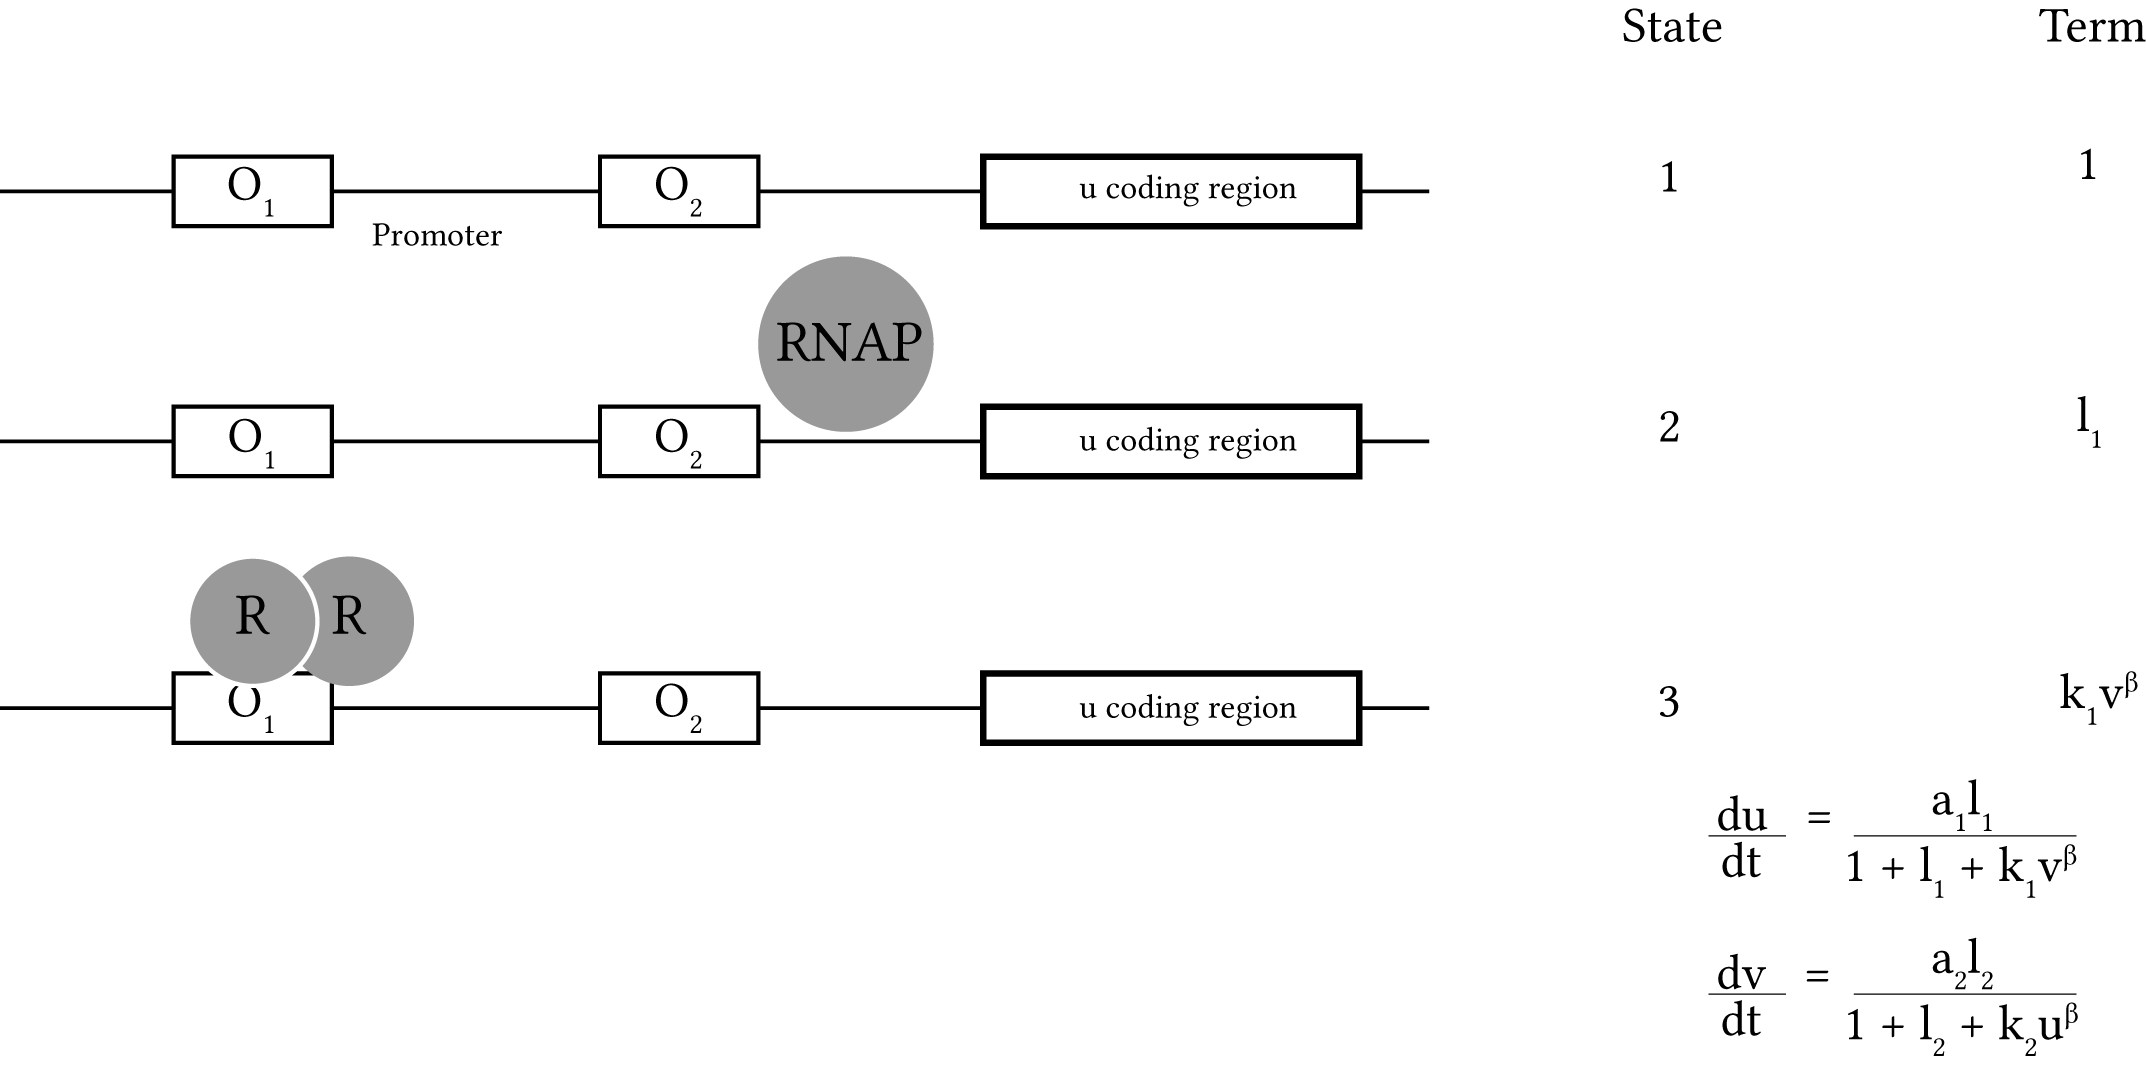
\includegraphics[scale=0.7]{../../chapters/chapterABCSysBio/images/shea-ackers-cs.png}
\caption[Simple toggle switch model using the Shea-Ackers formalism]{\label{fig:sa-GCS}Simple toggle switch model using the Shea-Ackers formalism}
\end{figure*}


\noindent The model can thus also be described by the following \acrshort{ode}s:

\begin{align}\label{eq:gards_sa}
\frac{du}{dt} &= \frac{a_1  l_1}{1 + l_1 + k_1  v^{\beta}} - u \\\label{eq:gards2_sa}
\frac{dv}{dt} &= \frac{a_2  l_2}{1 + l_2 + k_2  u^{\gamma }} - v,
\end{align}

The model shown in Equations~\ref{eq:gards1}-\ref{eq:gards2} is the dimensionless version of the model shown in Equations~\ref{eq:gards_sa}-\ref{eq:gards2_sa}. This is constructed by measuring $a_1$ and $a_2$ in units of $k_{1}^{\frac{-1}{β}}$ and $k_{2}^{\frac{-1}{γ}}$ respectively~\autocite{phys_biol_cell}. In the following section I will use the Shea-Ackers version of the model to show that it is also capable of bistable behaviour. 

\subsection{Phase space and bifurcation analysis}
\label{sec:bifurc}


First, I study the model given in Equations~\ref{eq:gards_sa}-\ref{eq:gards2_sa} by conducting a bifurcation analysis in order to confirm that it is capable of bistable behaviour. A bifurcation analysis is used to determine the properties of a system in parameter space~\autocite{Alon:2007}. Here I used the PyDSTool~\autocite{Clewley:2012kj}, a python package used for the analysis of dynamical systems. 


The parameters chosen here for the bifurcation analysis are within the range suggested by~\textcite{Gardner:2000vha}.  $a_1$ and $a_2$ are set to 10, and β, γ set to 2. A vector plot shows that the system has two steady states as shown in Figure~\ref{fig:Gard_CS}B. Both states were found to be stable by examining the eigenvalues of the system at each steady state using Mathematica~\autocite{mathematica:2016}.


I further study the system by conducting a bifurcation analysis, where all parameters remain constant to the values shown above, and only one parameter ($a_1$) is varied. The bifurcation analysis shows that by varying the parameter for the effective rate of synthesis of repressor 1 while all other parameters remain constant, the system is bistable when 5 \ge{} $a_1$ \le{} 31.



\begin{figure*}[htbp]
\centerfloat
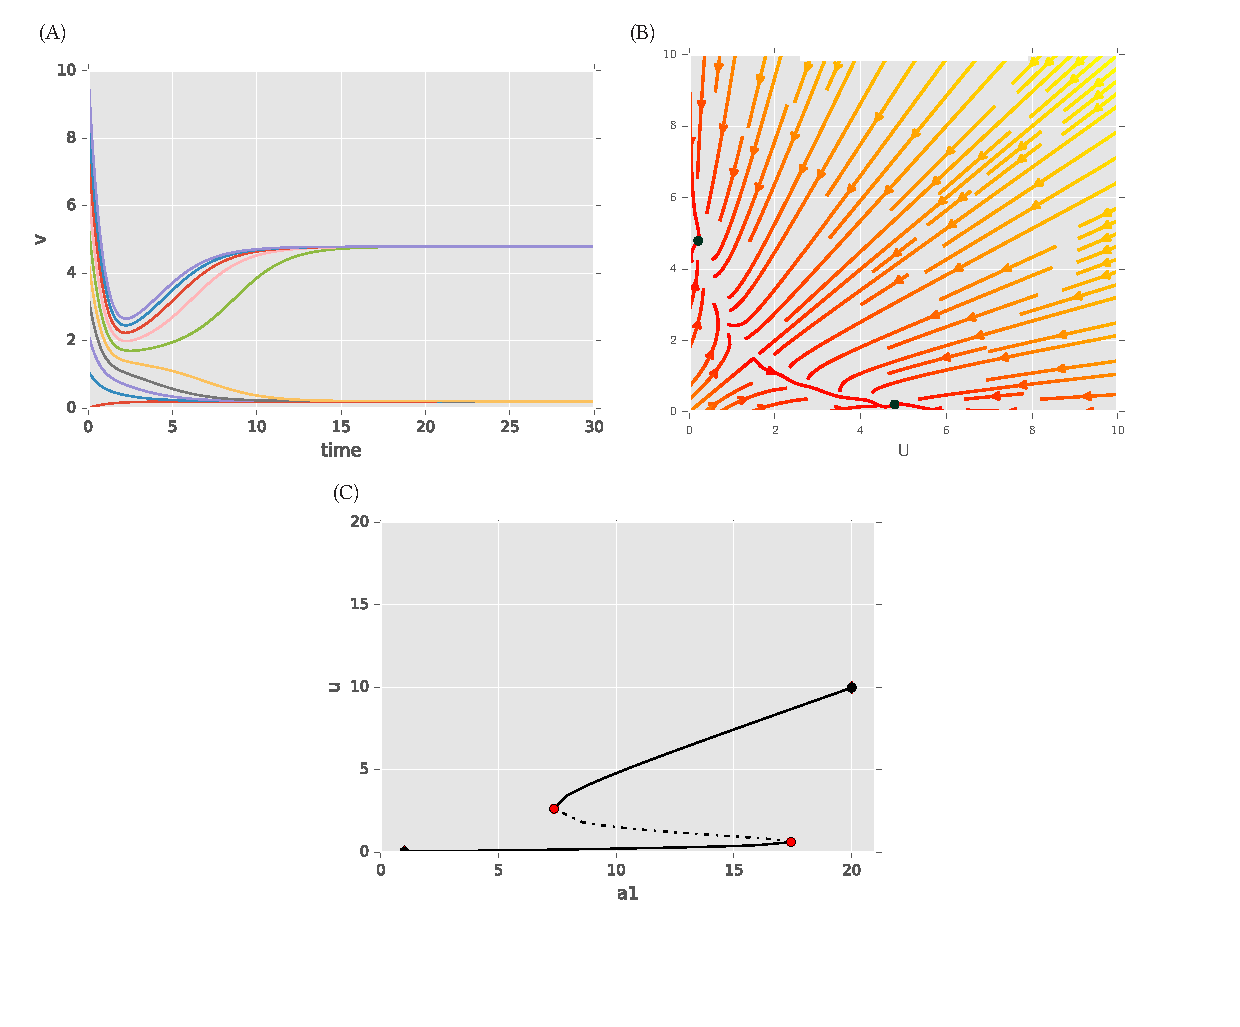
\includegraphics[scale=0.7]{../../chapters/chapterABCSysBio/images/Gard_CS.pdf}
\caption[Phase space and bifurcation analysis of the Gardner toggle switch]{\label{fig:Gard_CS}The \textcite{Gardner:2000vha} toggle switch is capable of bistable behaviour given $a_1$ and $a_2$ = 10, and β, γ = 2. (A) The time course of the simulated model using multiple initial conditions. (B) The vector plot of the Gardner switch shows there are two stable steady states. (C) A bifurcation diagram shows that the system is bistable when 5 \ge{} $a_1$ \le{} 31.}
\end{figure*}
\clearpage



\subsection{The quasi steady state approximation and the genetic toggle switch}
\label{sec:qssa}
In order for a system to be able to be studied mathematically, a number of assumptions have to be made. The system under consideration has to be reduced to very few equations and parameters in order to make the system solvable. This requires assumptions to be made about the system that cannot always be justified, such as the quasi-steady state approximation (QSSA). The QSSA assumes that the binding/unbinding processes are much faster than any other process~\autocite{Loinger:2007vma} thus the bound intermediate is assumed to always be in steady state. The QSSA assumption is met \textit{in vitro} but often does not hold \textit{in vivo}. Its misuse can lead to large errors and incorrectly estimated parameters~\autocite{Pedersen:2007ke}.

Equations~\ref{eq:gards1}-\ref{eq:gards2} of the genetic toggle switch can be derived from the full model by using the \acrfull{qssa}. In this Section I will discuss how Equations~\ref{eq:gards1}-\ref{eq:gards2} can be derived from the full model constructed under the mass action formalism by using the \acrshort{qssa}. Consider the set of reactions given in Table~\ref{tab:gard-qssa} representing the genetic toggle switch.

\begin{table}[h]
\centering
\caption{Toggle switch model reactions under mass action kinetics}
\label{tab:gard-qssa}
\begin{tabular}{@{}ll@{}}
\toprule
Equation                                                                             & Description                      \\ \midrule
${gu}\stackrel{{a_1}}{\longrightarrow}{gv} + {u}$                                             & \multirow{2}{*}{gene expression} \\
${gv}\stackrel{{a_2}}{\longrightarrow}{gu} + {v}$                                             &                                  \\
$β {u} \xrightleftharpoons[Kd_u]{Km_u}{u_β}$        & \multirow{2}{*}{dimerization}    \\
$γ {v} + {v} \xrightleftharpoons[Kd_v]{Km_v} {v_γ}$       &                                  \\
${gu} + {v_γ} \xrightleftharpoons[Kf_u]{Kr_u}{v_γ\bullet gu}$    & \multirow{2}{*}{repression}      \\
${gv} + {u_β} \xrightleftharpoons[Kf_v]{Kr_v}{u_β\bullet gv}$    &                                  \\
${u} \stackrel{{D_u}}{\longrightarrow}{\varnothing}$                     & \multirow{2}{*}{degradation}     \\
${v} \stackrel{{D_v}}{\longrightarrow}{\varnothing}$                     &                                  \\ \cmidrule(r){1-2}
\end{tabular}
\end{table}

\noindent Using mass action kinetics, this set of reactions gives us the following ODEs:

\begin{align}\label{eq:gard_ma_ode}
	\frac{du}{dt} &= a_{1}gu - Kd_{u}u^β + K_{m}u_β - D_u u\\
	\frac{dv}{dt} &= a_{2}gv - Kd_{v}v^γ + K_{m}v_γ - D_v v\\
	\frac{du_β}{dt} &= Kd_{u}u^β - Km_{u}u_β - Kf_{v}gv u_β\\
	\frac{dv_γ}{dt} &= Kd_{v}v^γ - Km_{v}v_γ - Kf_{u}gu v_γ\\
	\frac{dgu\bullet v_γ}{dt} &= Kf_{u}gv v_{γ} - Kr_{u}gu\bullet v_γ\\
	\frac{dgv\bullet u_β}{dt} &= Kf_{v}gu u_{β} - Kr_{v}gv\bullet u_β\\	
\end{align}


The principal quasi steady state assumption being made is that the rate of binding and unbinding of the repressor to the promoter happens very fast. We assume that it happens so much faster than any other reaction in the system that we can assume that $\frac{dgu\bullet v_γ}{dt}$ and $\frac{dgv\bullet u_β}{dt}$ are constant, i.e. in equilibrium. This assumption is also known as the separation of timescales in transcriptional regulation. In order for $\frac{dgu\bullet v_γ}{dt}$ and $\frac{dgv\bullet u_β}{dt}$ to be in equilibrium, we must assume that

\begin{align}
	\frac{dgu\bullet v_γ}{dt} &= Kf_{v}gv v_{γ} - Kr_{u}gu\bullet v_γ = 0\\
	\frac{dgv\bullet u_β}{dt} &= Kf_{u}gu u_{β} - Kr_{v}gv\bullet u_β = 0,
\end{align}

\noindent therefore,

\begin{align}
	Kf_{v}gv v_{γ} - Kr_{u}gu\bullet  v_γ &= 0\\
	Kf_{u}gu u_{β} - Kr_{v}gv\bullet  u_β &= 0,
\end{align}

\noindent Now we have a set of algebraic equations rather than differential equations. Solving for $\frac{dgu\bullet v_γ}{dt}$ and $\frac{dgv\bullet u_β}{dt}$  respectively we get:

\begin{align}
	gu\bullet  v_γ &= \frac{Kf_{v}gv v_{γ}}{Kr_{v}} \\
	gv\bullet  u_β &= \frac{Kf_{u}gu u_{β}}{Kr_{u}} 
\end{align}

\noindent This can now be substituted into the set of Equations~\ref{eq:gard_ma_ode}. The second assumption that is made in this system is that the rate of formation and dissociation of the polymerised transcription factor is in steady state. This allows us to solve the system for $u$ in a similar way as shown above and substitute it in Equations~\ref{eq:gard_ma_ode}. This results in a simplified model, with fewer differential equations and parameters.

\section{Designing a simple synthetic switch}
\label{sec:design_sim}
%This bit is from SF chapter as well

It was demonstrated that the model used in Section~\ref{sec:bifurc} is bistable for the parameters given. Nevertheless, for a switch to be useful in synthetic biological applications, it must be capable of behaving like a switch over a range of parameter values rather than just point values, as these fluctuate within the cellular environment. Therefore, in this section I study the parameter ranges that can give rise to a bistable switch. This indicates whether the bistability of the switch models is robust to small parameter fluctuations.


\subsection{Development of the mass action model for the genetic toggle switch}

In order to study the switch system in a more realistic way, I developed an extension to the ~\textcite{Gardner:2000vha} switch. This new set of switches does not use the \acrfull{qssa}, as described in Section~\ref{sec:qssa}. Avoiding the use of the \acrshort{qssa} the model becomes more flexible, and does not assume that the formation of the polymerized transciption factors is in steady state or that the association and dissociation of the transcription factors to the promoter is in steady state.  

Using mass action, this changes the two-equation system used in Equations~\ref{eq:gards1}-\ref{eq:gards2} into a system of 18 equations. The equations describing the system are shown below and illustrated in Figure~\ref{fig:Gard_MA}. The \acrshort{ode}s are given in Appendix~\ref{ap:ODEs}. The system consists of two genes, gA and gB. The products of the genes homodimerise and mutually repress each other. A symmetric model, where the parameters for equivalent reactions are set to be the same, was used for simplicity.

\begin{figure*}[tb]
	\begin{center}
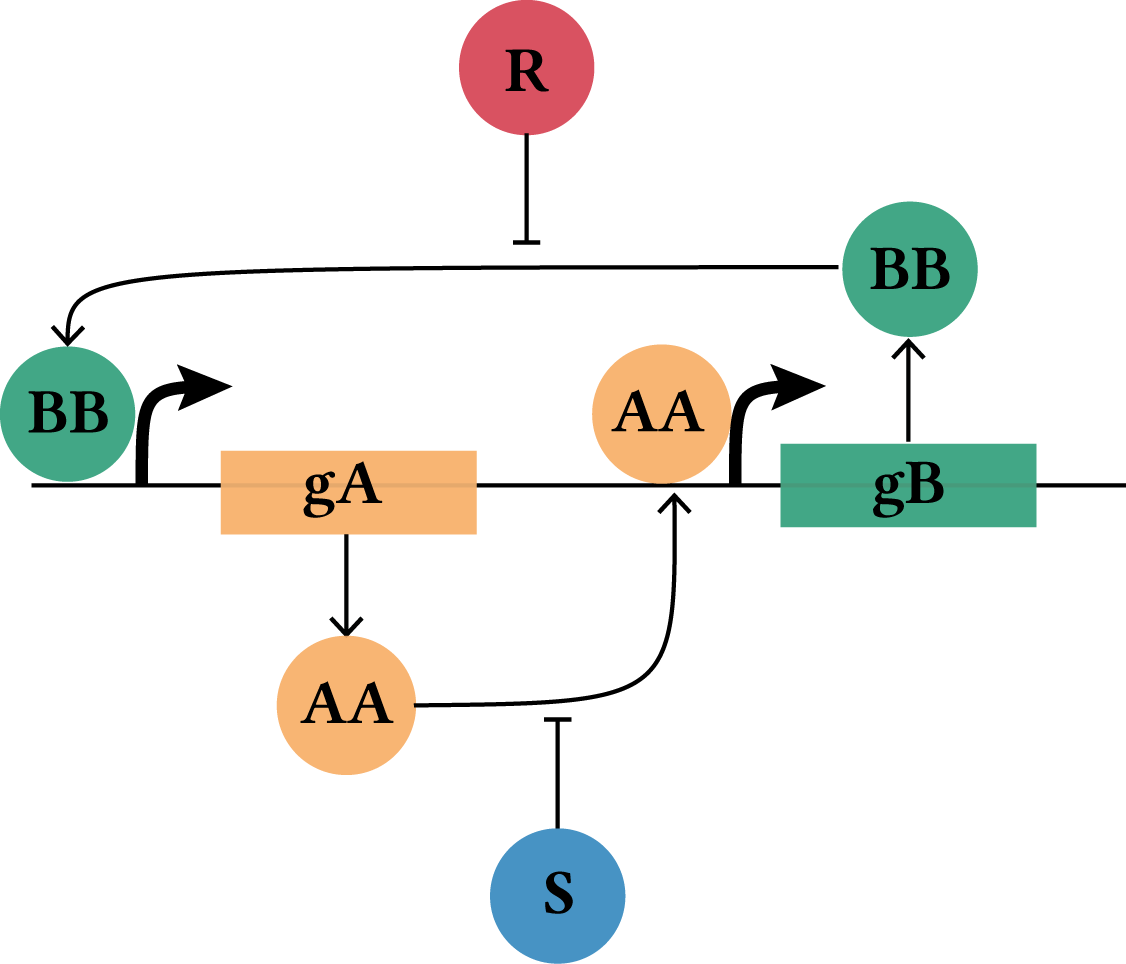
\includegraphics[scale=0.6]{../../chapters/chapterABCSysBio/images/ma-switch-diagram.png}
\caption[Toggle switch model used in the parameter scan]{\label{fig:Gard_MA}An illustration of the model used in the parameter scan. }
\end{center}
\end{figure*}



\begin{table}[tb]
\centering
\caption{Simple mass action switch reactions}
\label{tab:simp-ma-equ}
\begin{tabular}{@{}ll@{}}
\toprule
Equation                                                                             & Description                      \\ \midrule
$\textrm{gA}\stackrel{\textrm{ge}}{\longrightarrow}\textrm{gA} + \textrm{A}$                                             & \multirow{2}{*}{gene expression} \\
$\textrm{gB}\stackrel{\textrm{ge}}{\longrightarrow}\textrm{gB} + \textrm{B}$                                             &                                  \\
$\textrm{A} + \textrm{A} \stackrel{\textrm{dim}}{\longrightarrow}\textrm{A2}$        & \multirow{2}{*}{dimerization}    \\
$\textrm{B} + \textrm{B} \stackrel{\textrm{dim}}{\longrightarrow} \textrm{B2}$       &                                  \\
$\textrm{A2} \stackrel{\textrm{dim\_r}}{\longrightarrow}\textrm{A} + \textrm{A}$     & \multirow{2}{*}{monomerization}  \\
$\textrm{B2} \stackrel{\textrm{dim\_r}}{\longrightarrow}\textrm{B} + \textrm{B}$     &                                  \\
$\textrm{gA} + \textrm{B2} \stackrel{\textrm{rep}}{\longrightarrow}\textrm{B2gA}$    & \multirow{2}{*}{repression}      \\
$\textrm{gB} + \textrm{A2} \stackrel{\textrm{rep}}{\longrightarrow}\textrm{A2gB}$    &                                  \\
$\textrm{B2gA} \stackrel{\textrm{rep\_r}}{\longrightarrow}\textrm{B} + \textrm{gA}$  & \multirow{2}{*}{dissociation}    \\
$\textrm{A2gB} \stackrel{\textrm{rep\_r}}{\longrightarrow}\textrm{A2} + \textrm{gB}$ &                                  \\
$\textrm{A} \stackrel{\textrm{deg}}{\longrightarrow}\varnothing$                     & \multirow{2}{*}{degradation}     \\
$\textrm{B} \stackrel{\textrm{deg}}{\longrightarrow}\varnothing$                     &                                  \\ \cmidrule(r){1-2}
\end{tabular}
\end{table}

%$$
%\begin{array}{cccc}
%      \textrm{gA}\stackrel{\textrm{ge}}{\longrightarrow}\textrm{gA} + \textrm{A} \\
%      \textrm{gB}\stackrel{\textrm{ge}}{\longrightarrow}\textrm{gB} + \textrm{B} \\
%      \textrm{A} + \textrm{A} \stackrel{\textrm{dim}}{\longrightarrow}\textrm{A2} \\
%      \textrm{A2} \stackrel{\textrm{dim\_r}}{\longrightarrow}\textrm{A} + \textrm{A} \\
%      \textrm{B} + \textrm{B} \stackrel{\textrm{dim}}{\longrightarrow} \textrm{B2} \\
%      \textrm{B2} \stackrel{\textrm{dim\_r}}{\longrightarrow}\textrm{B} + \textrm{B} \\
%      \textrm{gA} + \textrm{B2} \stackrel{\textrm{rep}}{\longrightarrow}\textrm{B2gA} \\
%      \textrm{B2gA} \stackrel{\textrm{rep\_r}}{\longrightarrow}\textrm{B} + \textrm{gA} \\
%      \textrm{gB} + \textrm{A2} \stackrel{\textrm{rep}}{\longrightarrow}\textrm{A2gB} \\
%      \textrm{A2gB} \stackrel{\textrm{rep\_r}}{\longrightarrow}\textrm{A2} + \textrm{gB} \\
%      \textrm{A} \stackrel{\textrm{deg}}{\longrightarrow}\textrm{\O}\\
%      \textrm{B} \stackrel{\textrm{deg}}{\longrightarrow}\textrm{\O}\\
%%      \textrm{S} + \textrm{A2} \stackrel{\textrm{rep\_dim}}{\longrightarrow}\textrm{SA2}\\
%%      \textrm{SA2} \stackrel{\textrm{rep\_dim\_r}}{\longrightarrow}\textrm{S} + \textrm{A2}\\
%%      \textrm{R} + \textrm{B2} \stackrel{\textrm{rep\_dim}}{\longrightarrow}\textrm{RB2}\\
%%      \textrm{RB2} \stackrel{\textrm{rep\_dim\_r}}{\longrightarrow}\textrm{R} + \textrm{B2}\\
%%      \textrm{R} \stackrel{\textrm{deg}}{\longrightarrow} \textrm{\O}\\
%%      \textrm{S} \stackrel{\textrm{deg}}{\longrightarrow}\textrm{\O}\\
%\end{array}
%$$
\clearpage
\subsection{Parameter scan for model stability}
\label{sec:paramscan}

The bifurcation analysis carried out in Section~\ref{sec:bifurc} can give us the conditions for bistability of a model with respect to one parameter being varied while all the others remain constant. Here I want to determine the range of parameter values for which the above model is bistable without assuming a specific point value for any parameter. Therefore I developed a parameter scanning algorithm, that varies all the parameters in the model over a given range. The algorithm is outlined in Algorithm~\ref{alg:param_scan} below. This method involves the scan of parameter values as well as initial conditions for A2 and B2. Parameter values are sampled randomly from a uniform distribution, U(0, 10). Here, each set of samples will be referred to as a particle. For each particle, latin hypercube sampling is used to sample initial conditions~\autocite{MCKAY:2000vt}. The uniform priors of the two species in consideration represent a rectangular space, which is subdivided into equal parts. Then a random sample is drawn from each sub-part, as illustrated in Figure~\ref{fig:lhs}. This is used to ensure that the whole space is sampled uniformly. Latin hypercube sampling is done in two dimensions, in order to sample initial conditions for the two dimers, A2 and B2. All other species have fixed initial conditions, with $gA = 1$ and $gB = 1$ while all other species are equal to zero. 

\begin{algorithm}[htbp]
\caption{Parameter scan algorithm}
\label{alg:param_scan}
 \begin{algorithmic}[1]
    \Statex
	\State Select 100 sets of parameter values from a random uniform distribution between 0 and 10.
	\For{each set of parameter values}:
		
		\Let{step}{1}
		\For{i in range(0, 10)}
			\For{j in range(0, 10)}
				\State A2 sample = random sample from U(i, i + step) 
				\State B2 sample = random sample from U(j, j + step) 
			\EndFor
		\EndFor
	\For{ each set of initial conditions}
	\State Integrate ODEs of the model to t = 100 mins
	\State Let s = \{s1, s2, ..., s8\}, the values of al species at last time point
	\State Find roots of system using s as starting estimates 
	\EndFor
	\State Plot phase plot of roots for A2, B2
	\EndFor
  \end{algorithmic} 
\end{algorithm}

\begin{figure*}[ht]
\begin{center}
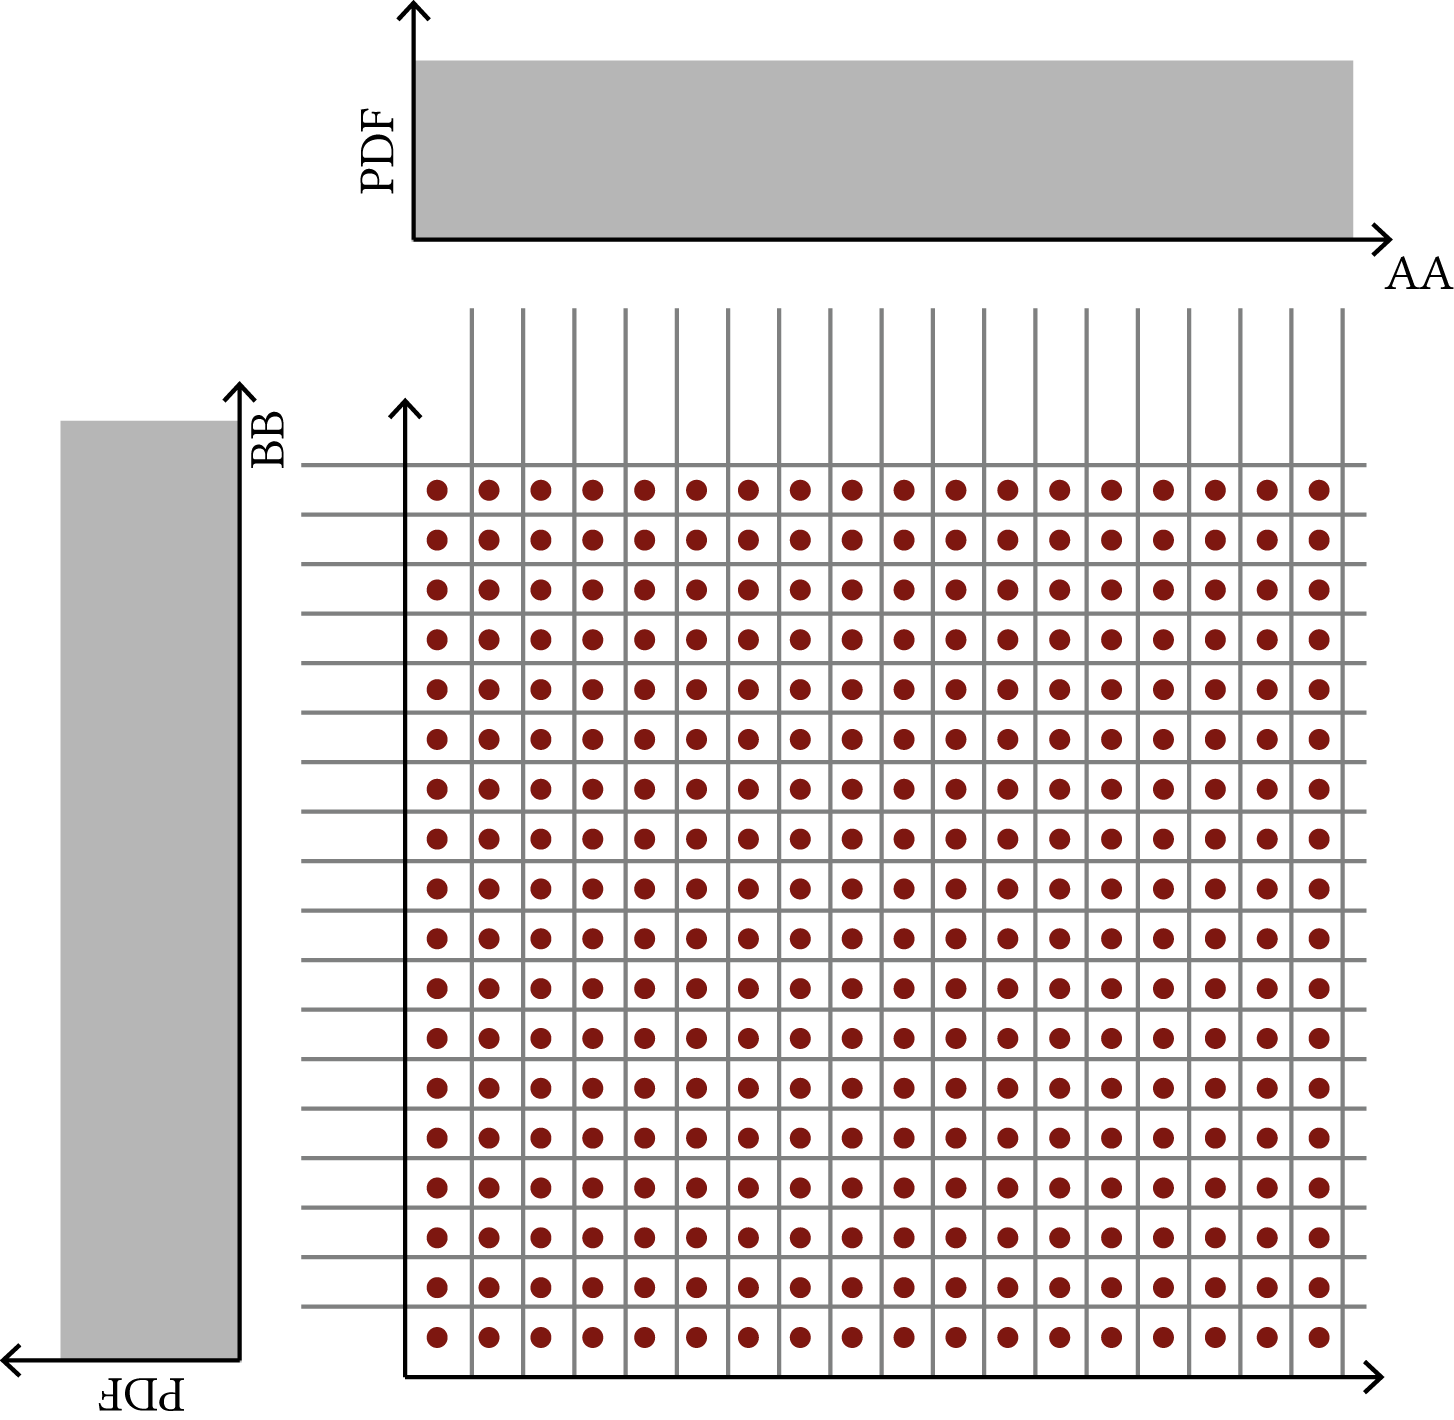
\includegraphics[scale=0.5]{../../chapters/chapterABCSysBio/images/LHS.png}
\caption[Latin Hypercube sampling]{\label{fig:lhs}Latin hypercube sampling ensures that the whole space is sampled evenly. For the two species concerned, A and B, we assume uniform distributions, shown in grey. The joint space of the two distributions is divided into smaller equal parts and a random sample is drawn from within each subspace.  }
\end{center}
\end{figure*}

The roots of each particle for each initial condition were found using the Python package SciPy~\autocite{Scipy}. A phase plot was made for each particle, which consists of the last time point value of one dimer plotted against the other. The parameter scan uncovered the presence of bistable and monostable systems given a different set of parameter values. An example of the phase plots for each of the three types of stabilities found during the scan are shown in Figure~\ref{fig:stab exampl}.

\begin{figure*}[htbp]
\centering
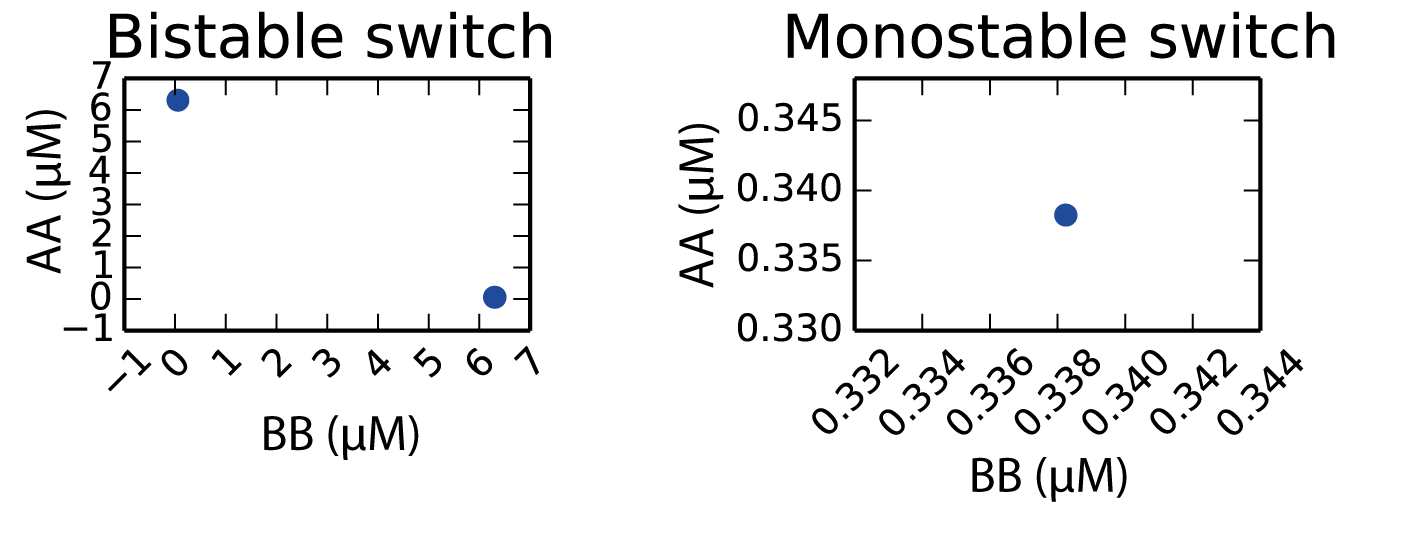
\includegraphics[width=0.7\textwidth]{../../chapters/chapterABCSysBio/images/phase_plots_param_scan.png}
\caption[Phase space examples of a monostable and a bistable switch]{\label{fig:stab exampl}An example for each type of switch found during the parameter scan. Each graph represents the steady state values of one dimer plotted against8the other, from one parameter set and 100 initial conditions.}
\end{figure*}

A total of 1000 parameter sets were sampled. Out of these, 56\% were monostable, 35.2\% did not reach steady state and 8.8\% where bistable. The distributions of the parameters that produced each stability are shown in Figure~\ref{fig:scan ode param hist}. 

\begin{figure}
\centering
\begin{minipage}[c]{1\textwidth}
\centering
    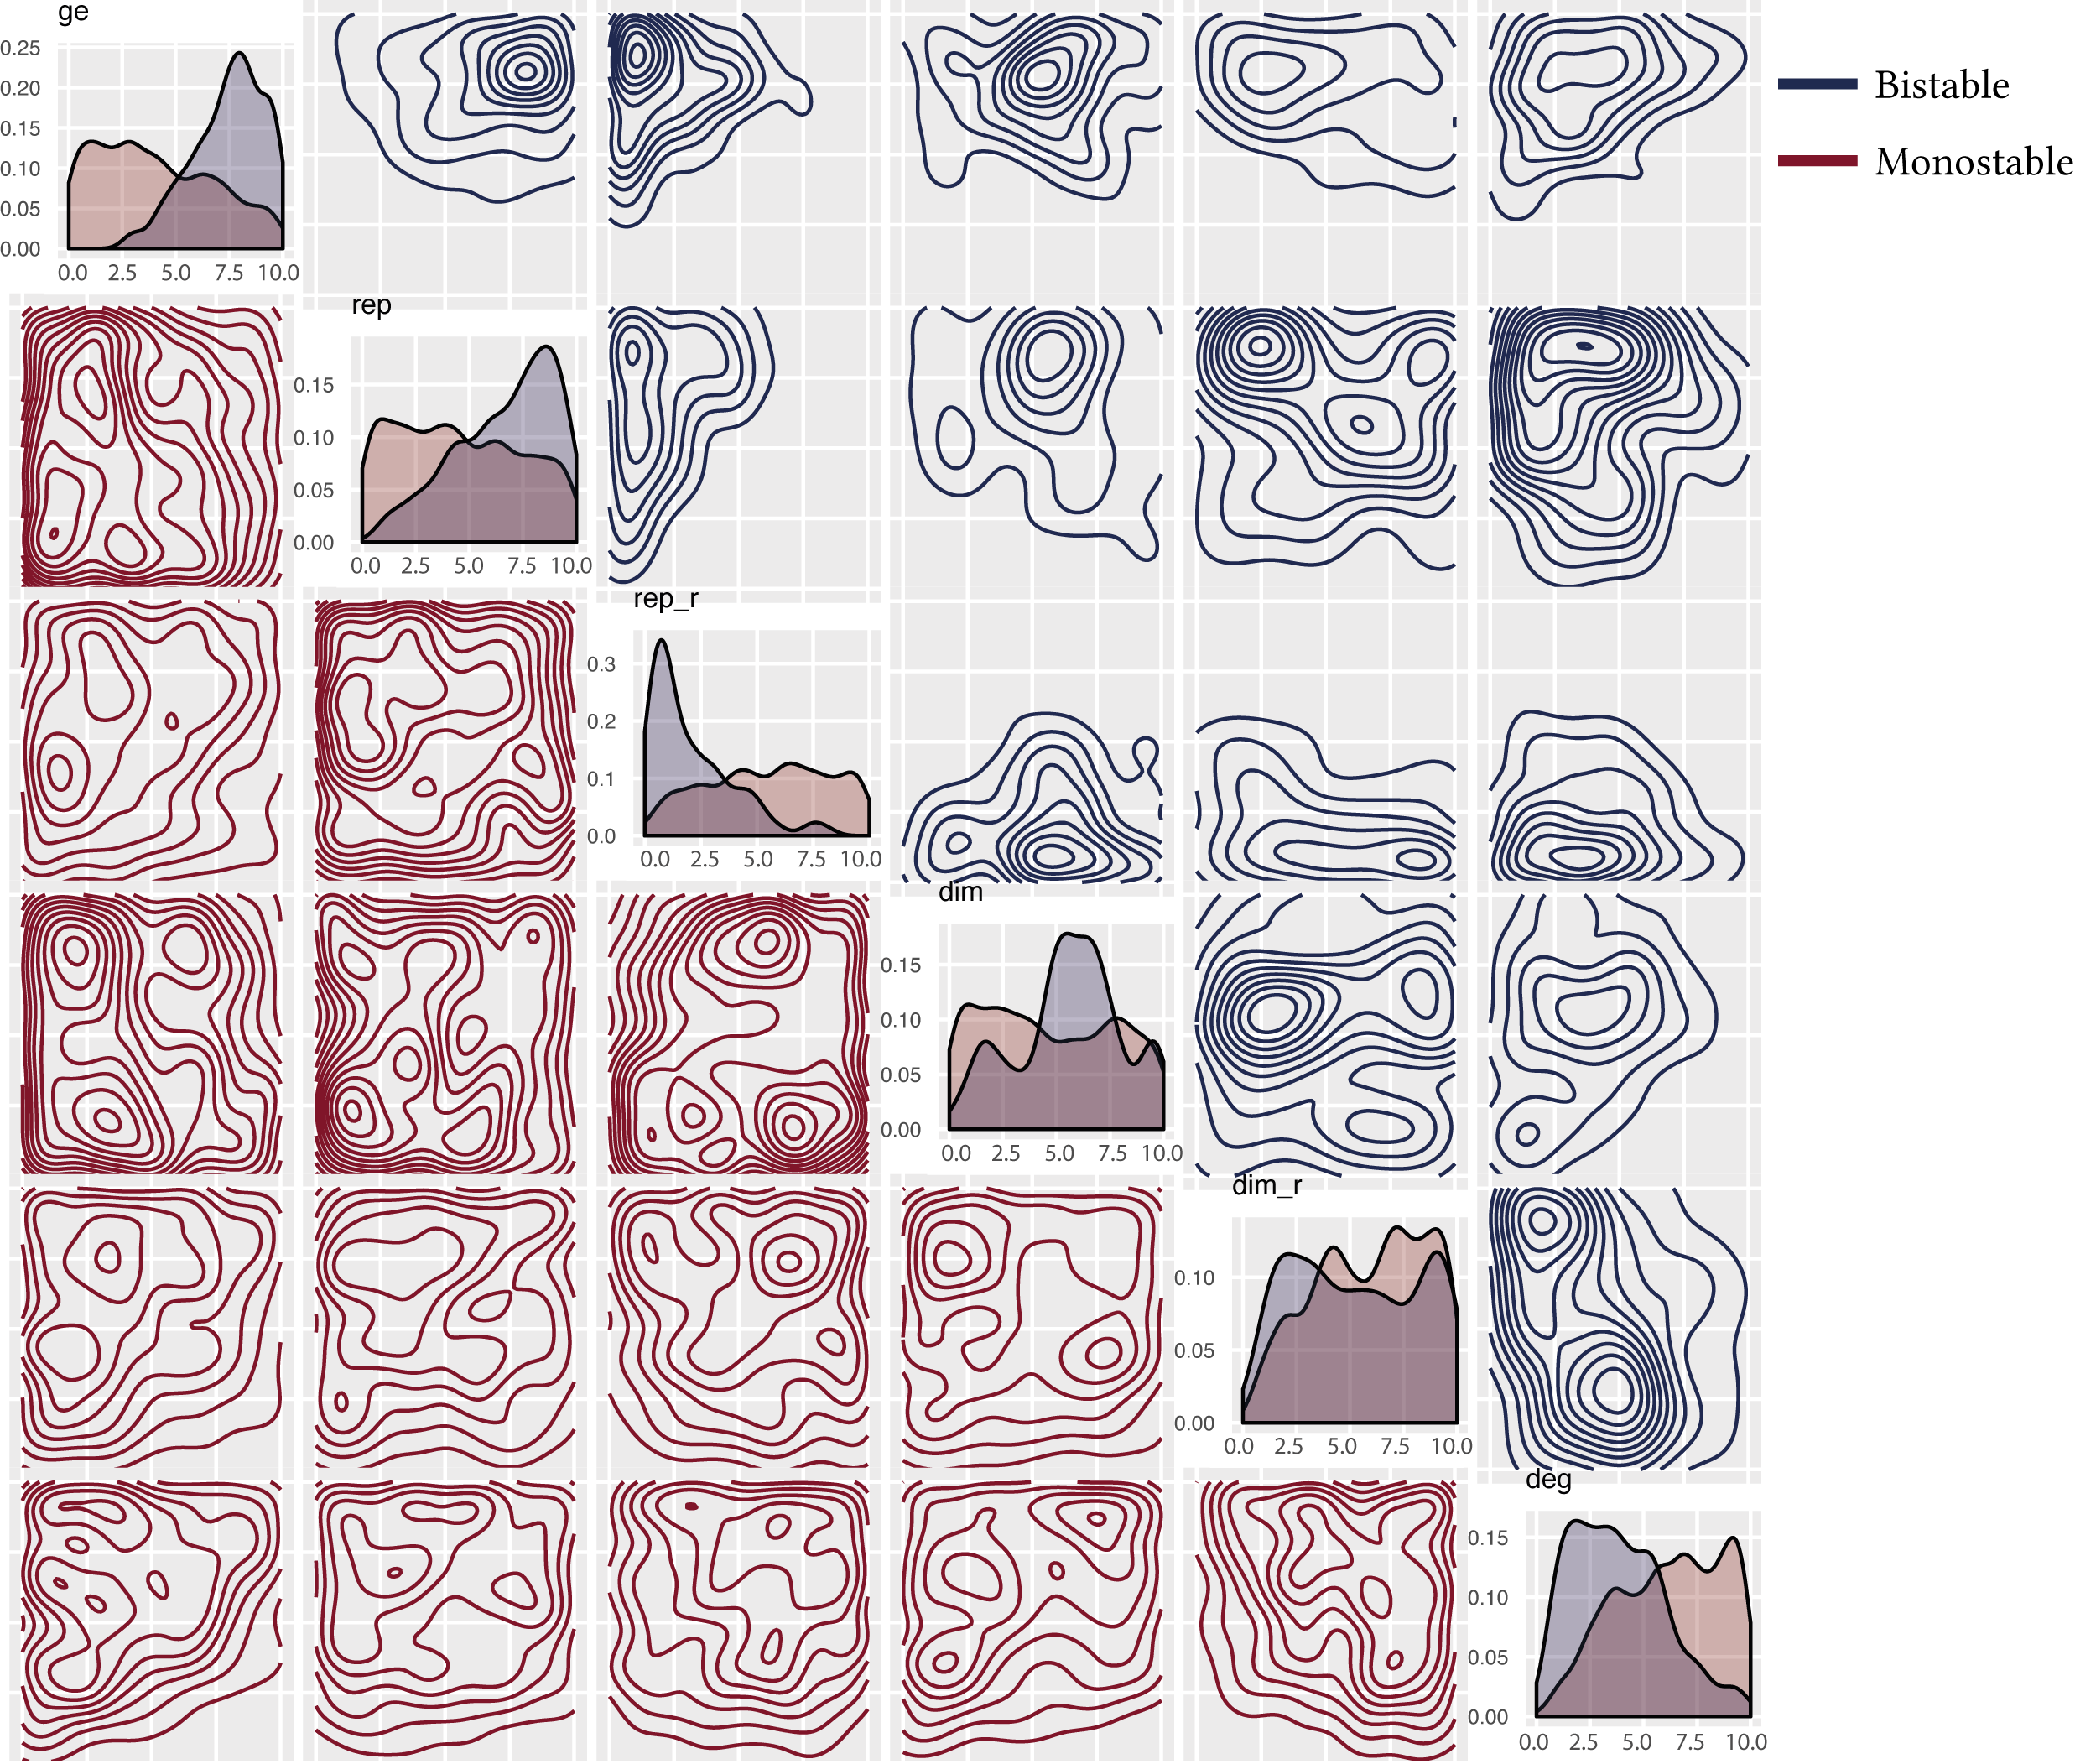
\includegraphics[width=1.2\textwidth]{../../chapters/chapterABCSysBio/images/param_scan_combo.png}
    \caption[Distributions of the parameters resulting in each stability obtained by the parameter scan]{The distribution of parameter values that resulted in monostable and bistable switches in the parameter scan. The one-dimensional marginal distribution of each parameter is plotted on the diagonal and the the two-dimensional marginal distributions are on the off-diagonal. }
    \label{fig:scan ode param hist}
\end{minipage}
\end{figure}


From Figure~\ref{fig:scan ode param hist} it can be seen that the parameter for gene expression (ge) tends to be relatively high when bistability arises. The parameter for repression (rep) tends to be high whereas the parameter for its reverse reaction (rep\_r) tends to be low. From this analysis I showed that the toggle switch is capable of bistable behaviour for a range of parameter values. 

\subsection{Toggle switch parameter inference}
\label{sec:param_inf}
In this section, I extend the analysis carried out in Section~\ref{sec:paramscan} to study the problem of how to rationally design a synthetic biological system to perform a behaviour of choice.  In order to address this question I use a Bayesian approach, known as \acrlong{abc} and described in Section~\ref{sec:abc}, implemented in a software package, ABC-SysBio~\autocite{Liepe:2010eg}. 

This approach is capable of approximating the posterior distribution that gives rise to the behaviour of choice~\autocite{Toni:2009tr}. By simulating the model in question, this approach can identify an approximate posterior distribution via a series of intermediate distributions. This method can be used for the rational design of synthetic biological systems by defining some design objectives to which the model is fitted to~\autocite{Barnes:2011hh}. By specifying the inputs to the system and the outputs required, the posterior of the model that can produce this behaviour can be identified. 

Here I use ABC-SysBio to fit a model to the design objectives of a switch-like behaviour. I extend the model used in Section~\ref{sec:paramscan} by adding two inducers to the system, S and R. S removes the A homodimer (A2) from the system by binding to it thus removing the repression on gene B. R removes B2 from the system with the same mechanism. These inducers represent the stimuli that will turn the switch ON and OFF in a biological setting. The following equations are added to the existing set of equations for the mass action switch: 

\begin{table}[htbp]
\centering
\caption{Toggle switch inducer equations}
\label{tab:toglle-inducer-equs}
\begin{tabular}{@{}ll@{}}
\toprule
Equation                                                                                & Description                           \\ \midrule
$\textrm{S} + \textrm{A2} \stackrel{\textrm{rep\_dim}}{\longrightarrow}\textrm{SA2}$    & \multirow{2}{*}{Inducer repression}   \\
$\textrm{R} + \textrm{B2} \stackrel{\textrm{rep\_dim}}{\longrightarrow}\textrm{RB2}$    &                                       \\
$\textrm{SA2} \stackrel{\textrm{rep\_dim\_r}}{\longrightarrow}\textrm{S} + \textrm{A2}$ & \multirow{2}{*}{Inducer dissociation} \\
$\textrm{RB2} \stackrel{\textrm{rep\_dim\_r}}{\longrightarrow}\textrm{R} + \textrm{B2}$ &                                       \\
$\textrm{R} \stackrel{\textrm{deg}}{\longrightarrow} \varnothing$                       & \multirow{2}{*}{Inducer degradation}  \\
$\textrm{S} \stackrel{\textrm{deg}}{\longrightarrow}\varnothing$                        &                                       \\ \cmidrule(r){1-2}
\end{tabular}
\end{table}
%$$
%\begin{array}{cccc}
%      \textrm{S} + \textrm{A2} \stackrel{\textrm{rep\_dim}}{\longrightarrow}\textrm{SA2}\\
%      \textrm{SA2} \stackrel{\textrm{rep\_dim\_r}}{\longrightarrow}\textrm{S} + \textrm{A2}\\
%      \textrm{R} + \textrm{B2} \stackrel{\textrm{rep\_dim}}{\longrightarrow}\textrm{RB2}\\
%      \textrm{RB2} \stackrel{\textrm{rep\_dim\_r}}{\longrightarrow}\textrm{R} + \textrm{B2}\\
%      \textrm{R} \stackrel{\textrm{deg}}{\longrightarrow} \textrm{\O}\\
%      \textrm{S} \stackrel{\textrm{deg}}{\longrightarrow}\textrm{\O}\\
%\end{array}
%$$
The range of parameter values shown to produce a bistable switch in Section~\ref{sec:paramscan} were used as priors and are shown in Table~\ref{tab:param_inf_params}. Initial conditions of the two genes, $gA$, $gB$ were set to 1, and species $A$ and $A2$ were set to 50 and 10 respectively, in order to set the starting conditions of the switch to $B2$ OFF. All other species initial conditions were set to 0. 

\begin{table}[t]
\centering
\caption{The prior distributions used for the standard toggle switch parameter inference. The values indicate the lower and upper limits (inclusive) of a uniform distribution.}
\label{tab:param_inf_params}
\centerfloat
\resizebox{1.3\textwidth}{!}{\begin{tabular}{cccccccccc}
\toprule
 \textbf{ge}     & \textbf{rep}     & \textbf{rep\_r}     & \textbf{dim}    & \textbf{dim\_r}     & \textbf{deg}  & \textbf{rep\_dim}    & \textbf{rep\_dim\_r} & \textbf{deg\_sr} & \textbf{deg\_dim}   \\
 (min\textsuperscript{-1})&(μM min\textsuperscript{-1})&(min\textsuperscript{-1})&(μM min\textsuperscript{-1})&(min\textsuperscript{-1})&(min\textsuperscript{-1})&(μM min\textsuperscript{-1})&(min\textsuperscript{-1})&(min\textsuperscript{-1})&(min\textsuperscript{-1})\\
6-9     & 4-10    & 1-4       & 4-10   & 2-7       & 2-5  & 0.05-0.1   & 0.01-0.05     & 0.01-0.05  & 0-1      \\ \bottomrule
\end{tabular}}
\end{table}

\subsection{Design specifications}

The following were defined as the design specifications for a bistable genetic toggle switch. The two inducers, S and R, are used as inputs to flip the switch ON and OFF respectively. The required output is the switch flipping from the OFF state to the ON state and then to the OFF state again (Figure~\ref{fig:abc_behav}). 


\begin{figure*}[htbp]
	\begin{center}
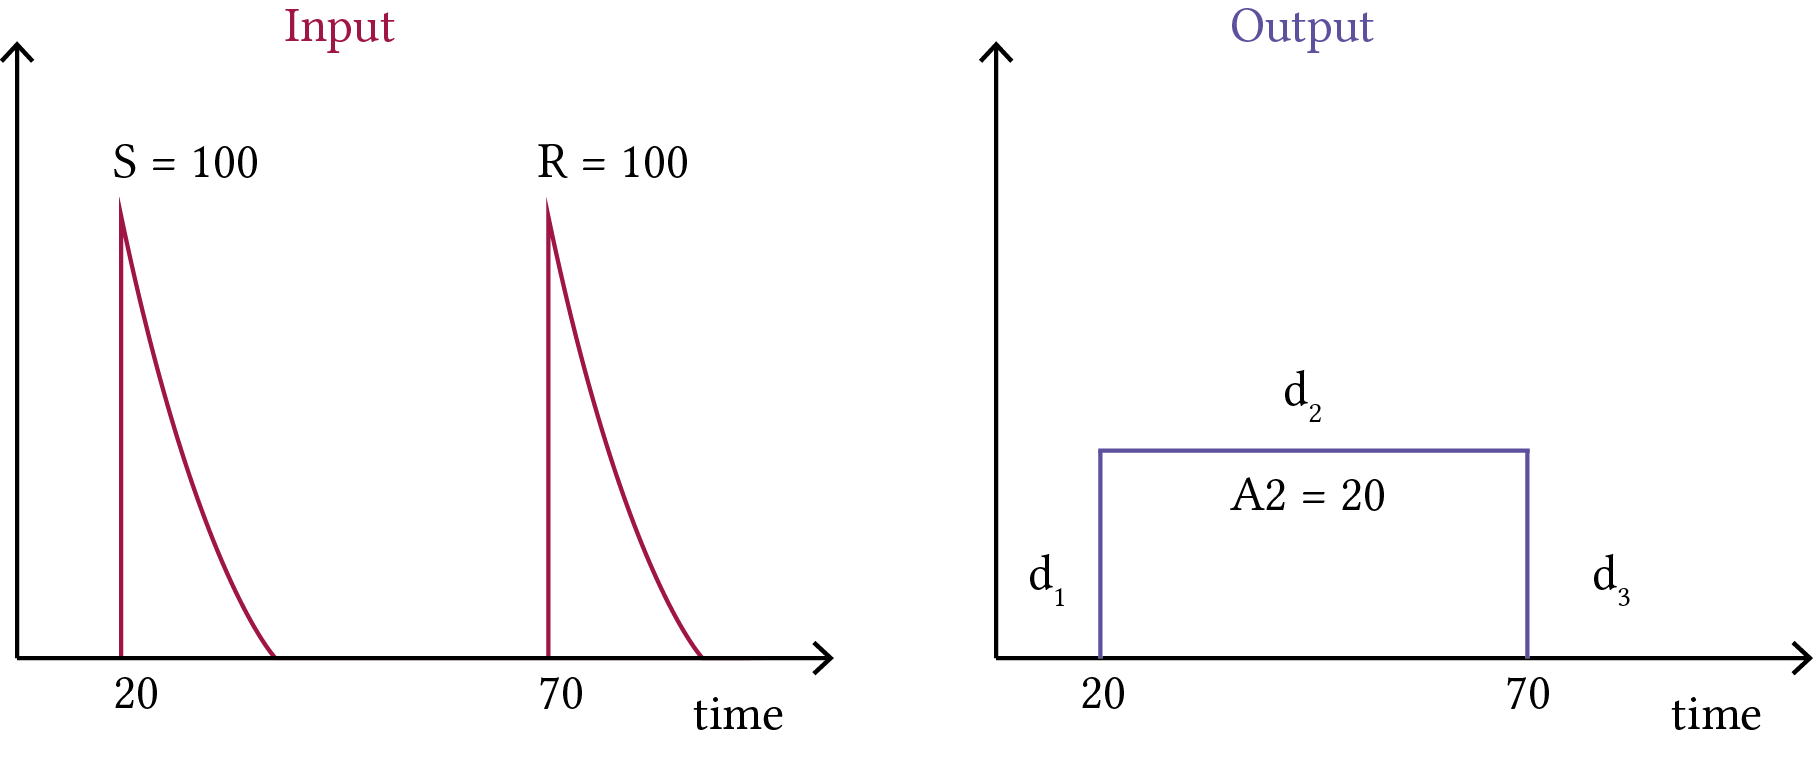
\includegraphics[scale=0.7]{../../chapters/chapterABCSysBio/images/behaviour.png}
\caption[Design specification for ABC parameter inference]{\label{fig:abc_behav}Design specification for ABC parameter inference. The input to the system consists of an event turning on the stimulus (S) at t=20 and another turning on the repressor (R) at t=70. The output specification is the response to the switch to these stimuli.}
\end{center}
\end{figure*}

\subsubsection{Distance function}
In order to fit the switch model to the behaviour specified above, a distance function must be defined. The distance function defines the quantity that is minimized at each successive iteration of \acrshort{abc} \acrshort{smc}. Three distances are measured, one for each state of the switch, OFF-ON-OFF. Each distance is the sum of the distances of the simulated protein levels to the desired protein levels at each time point. All three distances must reach the minimum threshold for the process to be complete. 

\begin{align}\label{eq:dist}
	d_1 &= \sum_{i=0}^{20} (s_i-t_1)^2 \\
	d_2 &= \sum_{i=21}^{70} (s_i-t_2)^2 \\
	d_3 &=  \sum_{i=71}^{100} (s_i-t_3)^2,
\end{align}
where $i$ represents the time points, $s_i$ the simulation result at  each time point and $t_1$, $t_2$, $t_3$ represent each target behaviour. $t_1$, $t_2$, $t_3$ were set to 0, 20, 0 respectively. 



\subsection{Results}

The results of the parameter inference of the toggle switch are shown in Figure~\ref{fig:stand_abc_timeseries}. The model was shown to successfully behave like a switch within the parameter range used here. The resulting time course of the last population matches the design specifications. It can be seen from the posterior distribution that gene expression rate (ge) must be high relative to the prior. Repression (rep) and degradation must both be low and the rate of dimerisation (dim) must be high relative to the prior. The posterior constitutes the specifications that can be used when building a synthetic switch in the lab, as the appropriate components can be tweaked for a successful circuit. More generally, the posterior distribution shows that the parameter space that can give rise to this behaviour is limited. A very small portion of the prior is capable of producing the desired design specifications. In the next section I will examine whether the addition of feedback loops can increase the robustness of this behaviour.


\begin{figure}[htbp]
    \centering
    \hspace*{-1cm}
    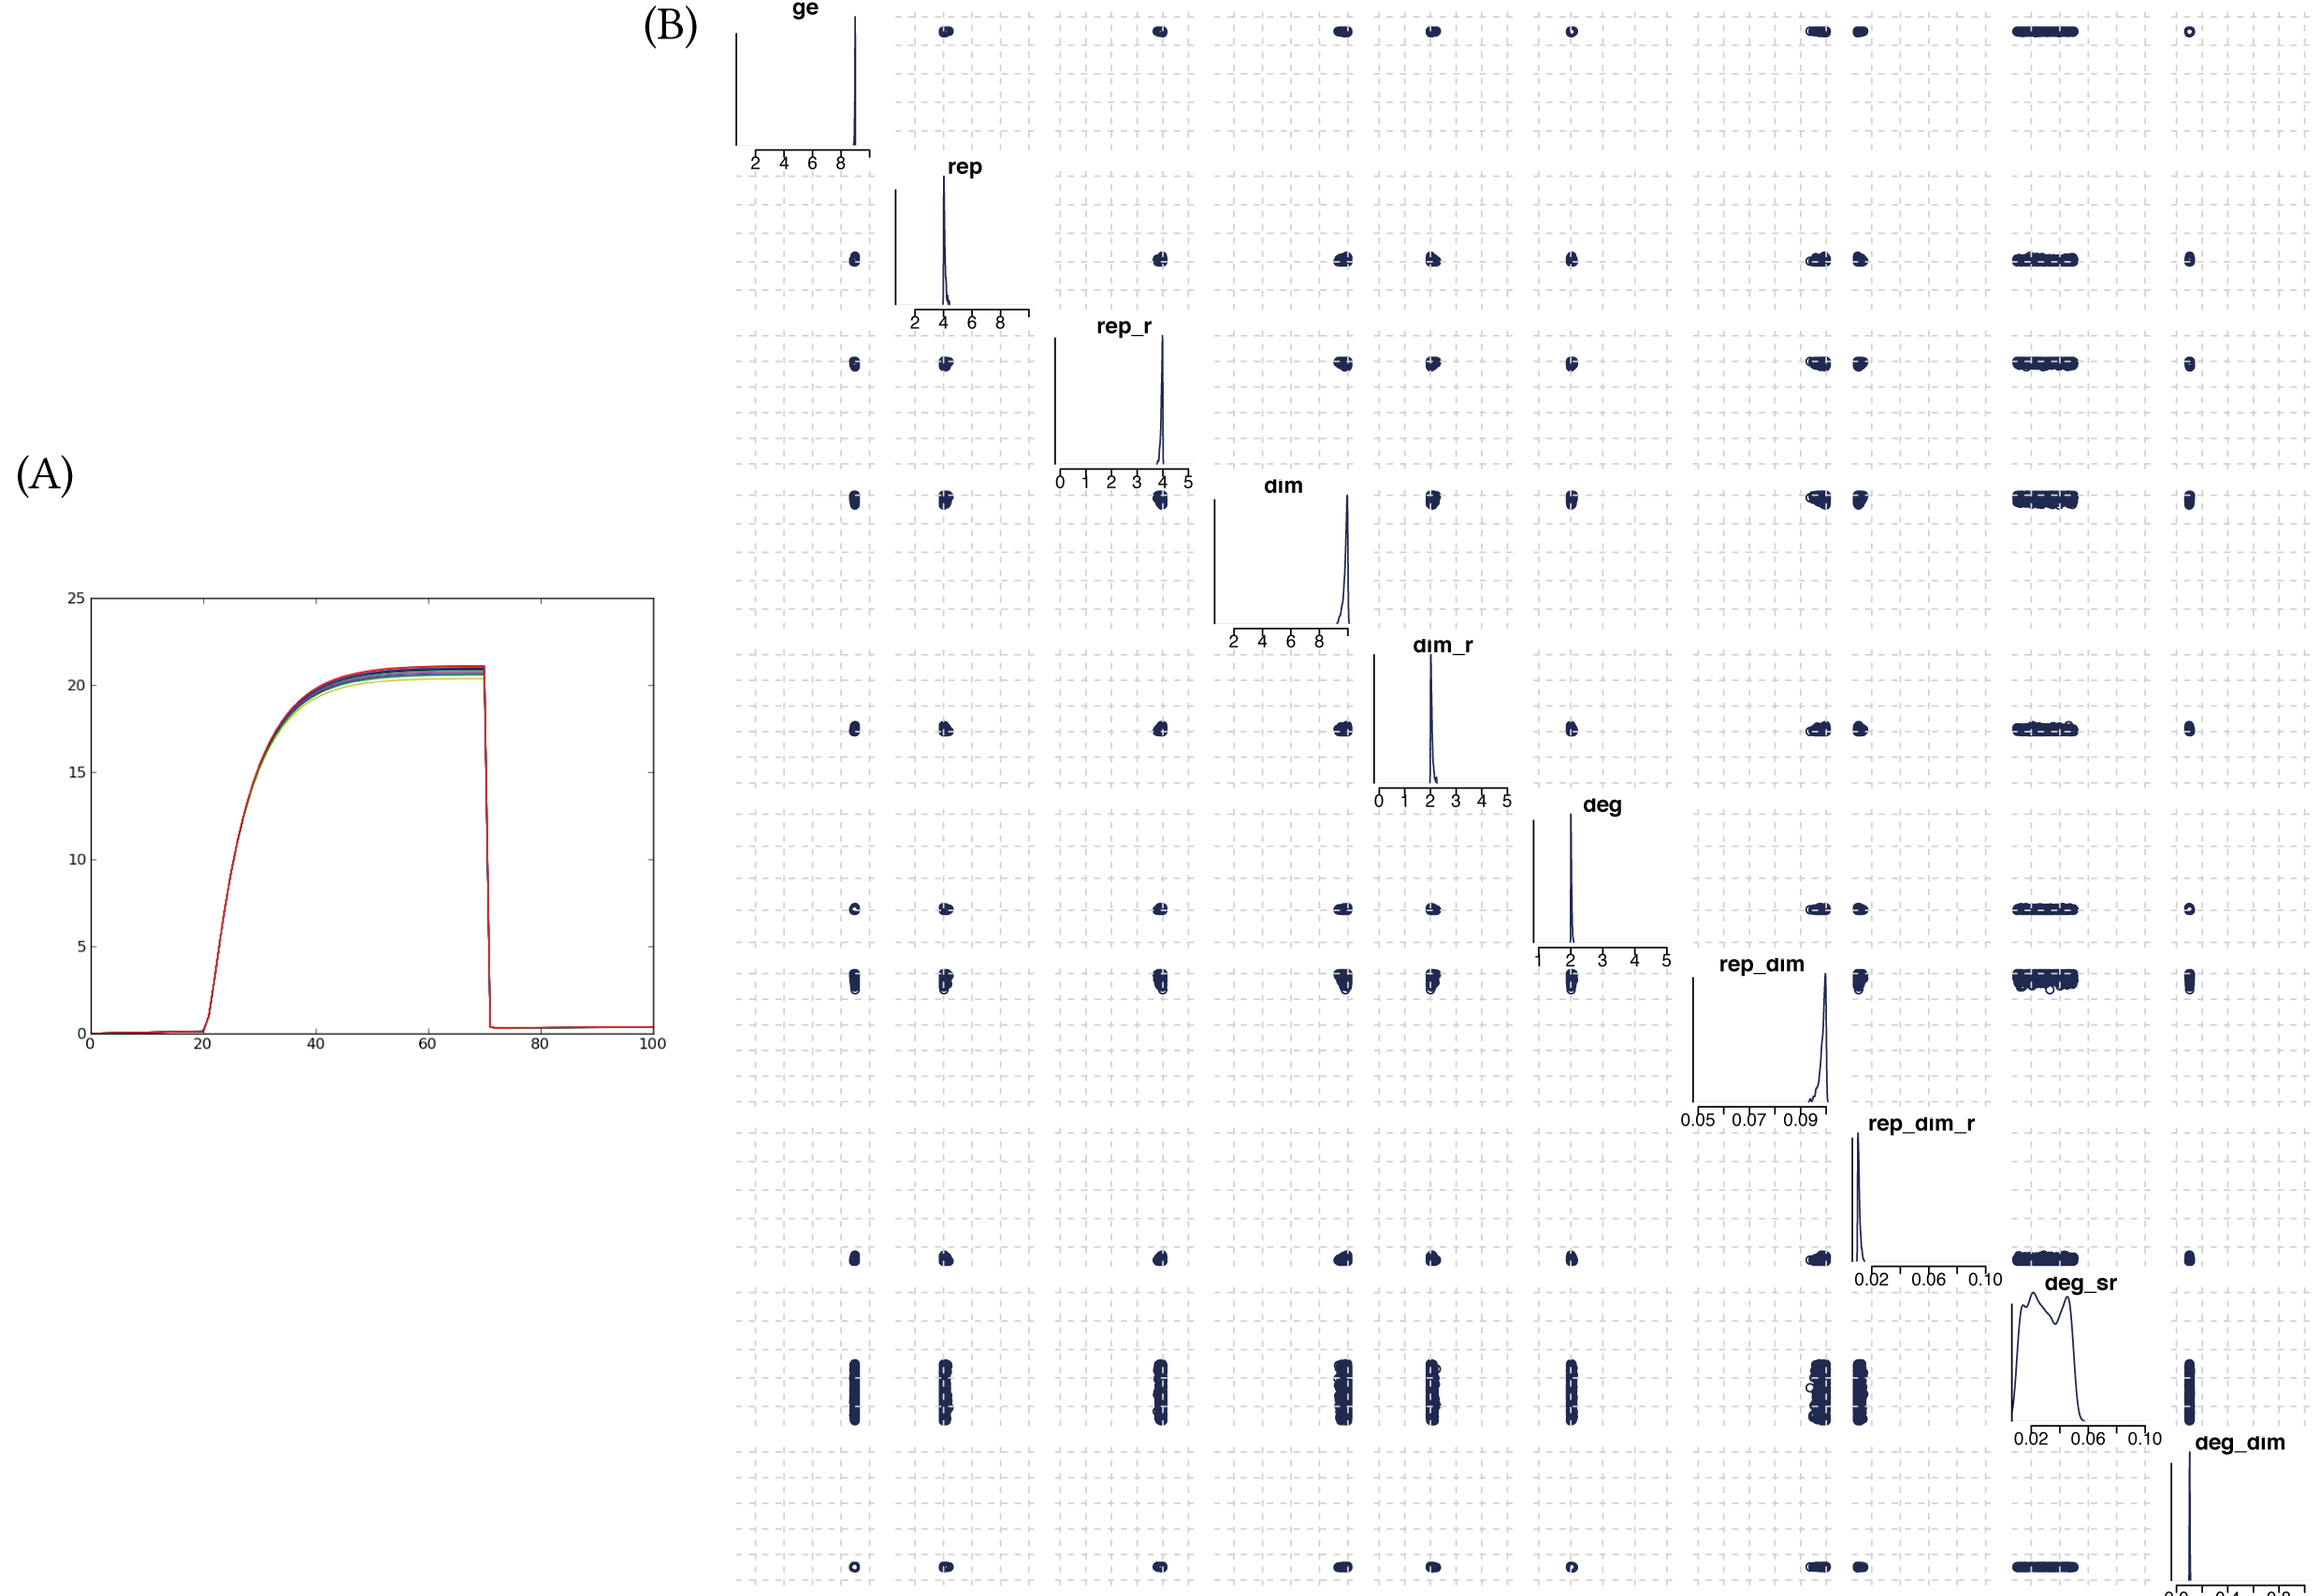
\includegraphics[scale=0.7]{../../chapters/chapterABCSysBio/images/param_inf_res.png}
    \caption[Posterior distribution of the switch obtained from ABC system design]{(A) The time series of the final population (for final $\epsilon$ = 2 ) of the standard toggle switch ABC-SMC parameter inference. The stimulus, that represses A2, is added at t=20 and the repressor, that represses B2 is added at t=70. (B) The posterior distribution of the toggle switch.}
    \label{fig:stand_abc_timeseries}
\end{figure}
\clearpage
    

\section{Designing a more robust genetic toggle switch}

In this section I examine whether the addition of feedback loops to the toggle switch can increase its robustness to parameter fluctuations. Here I define a robust system as a device that can withstand fluctuations in parameter values and still produce the desired behaviour (parametric robustness). Feedback loops are well known key regulatory motifs~\autocite{Brandman:2005ci}. 

As was shown in Section~\ref{sec:design_sim}, the posterior distribution of the simple toggle switch was narrow, and thus the behaviour of choice will not be robust. Here I examine whether adding feedback loops to the genetic toggle switch can increase parametric robustness for the desired design specifications.

\subsection{Models of the genetic toggle switch}
\label{sec:models_bist}

Both positive and negative feedback loops were considered. Therefore 7 models were examined for their capability to behave like a switch. The simple toggle switch, switches with positive autoregulation in either or both nodes and switches with negative autoregulation in either or both nodes. The models considered are illustrated in Figure~\ref{fig:toggle_switch_designs}. 

 In order to study each model mathematically I built extensions to the ~\autocite{Gardner:2000vha} toggle switch in order to incorporate positive and negative feedback to the system. These were constructed using the Shea-Ackers formalism, as described in Section~\ref{sec:shea-ackers}, as shown in Figure~\ref{fig:sa-autoreg}. The models for the double autoregulation models are shown below. For the single autoregulation models, the unnecessary autoregulation term is set to 0.


\begin{figure*}[tb]
\centerfloat
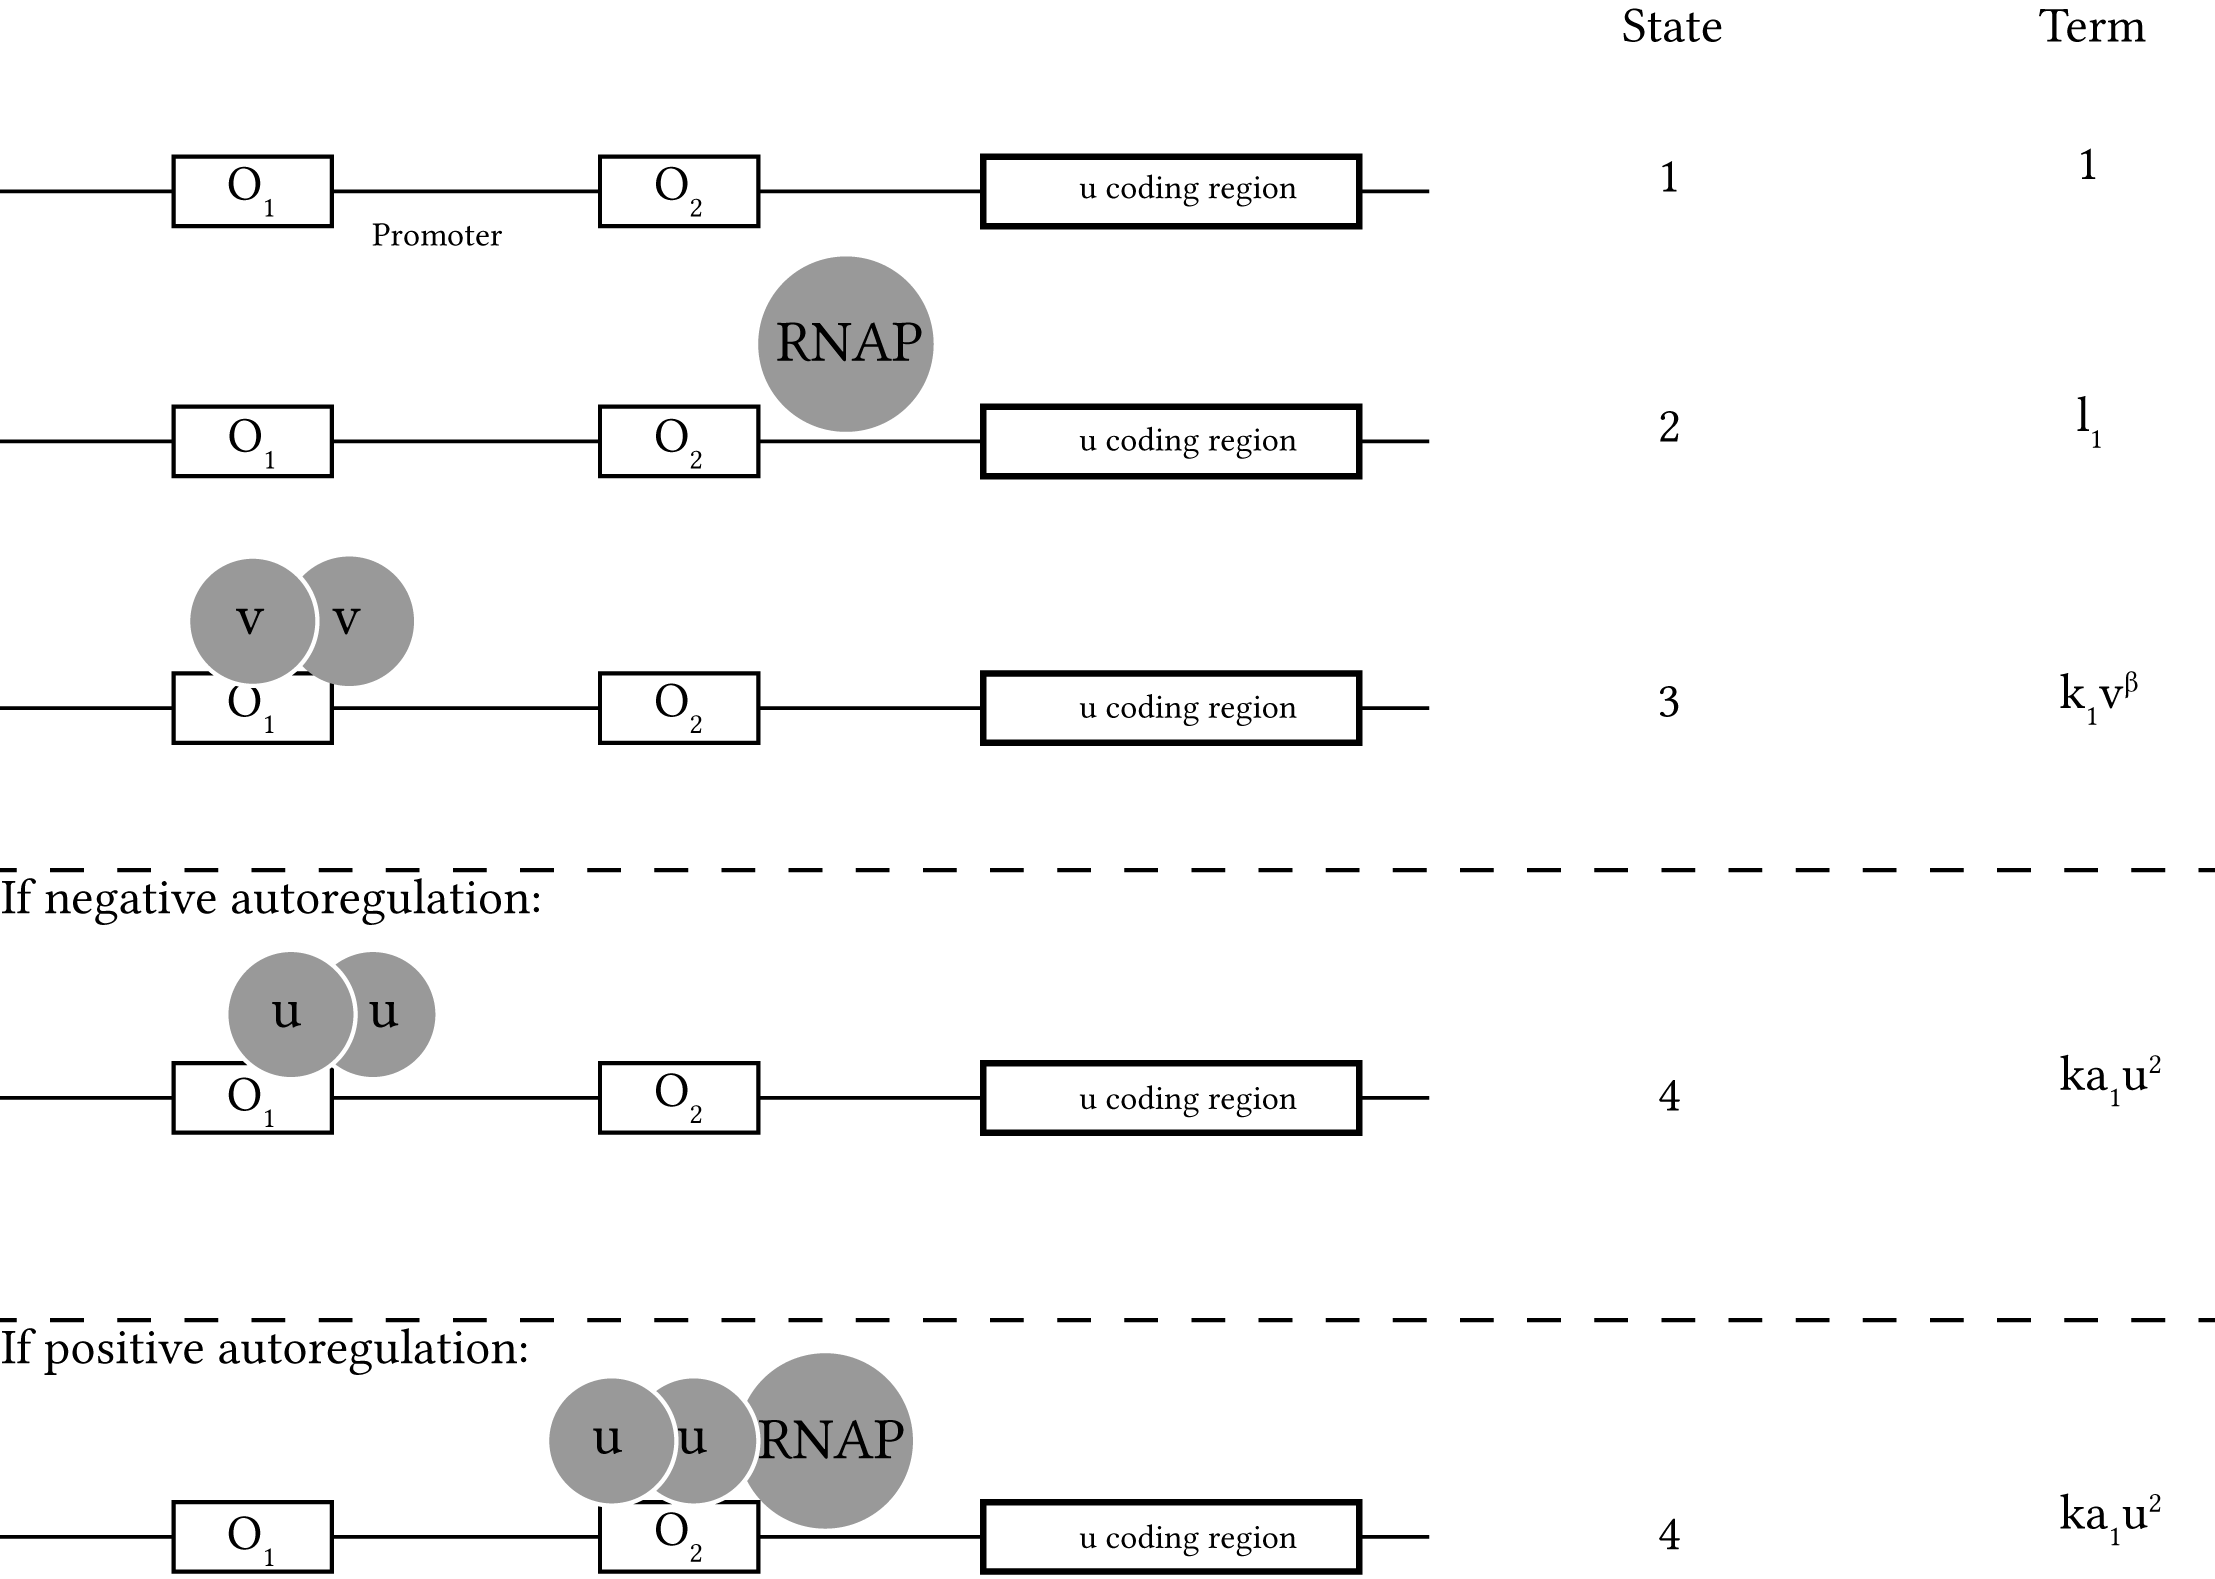
\includegraphics[scale=0.7]{../../chapters/chapterABCSysBio/images/shea-ackers_autoreg.png}
\caption[Toggle switch models with autoregulation using the Shea-Ackers formalism]{\label{fig:sa-autoreg}Toggle switch models with autoregulation using the Shea-Ackers formalism}
\end{figure*}



\noindent Double negative autoregulation: 
\begin{align}\label{eq:gards_neg}
\frac{du}{dt} &= \frac{a_1  l_1}{1+l_1+k_1  v^{\beta} + ka_{1}  u^{2}} - u \\
\frac{dv}{dt} &= \frac{a_2  l_2}{1+l_2+k_2  u^{\gamma }+ ka_{2}  v^{2}} - v,
\end{align}

\noindent Double positive autoregulation: 
\begin{align}\label{eq:gards_pos}
\frac{du}{dt} &= \frac{a_1  (l_1 + ka_{1}  u^{2}) }{1+l_1 + k_1  v^{\beta} + ka_{1}  u^{2}} - u \\
\frac{dv}{dt} &= \frac{a_2  (l_2 + ka_{2}  v^{2}) }{1+l_2 + k_2  u^{\gamma} + ka_{2}  v^{2}} - v,
\end{align}

\noindent where $k$ represents the effective binding of the transcription factor to its own promoter and β, γ represent the polymerisation of the bound transcription factors. 


\begin{figure*}[tb]
	\begin{center}
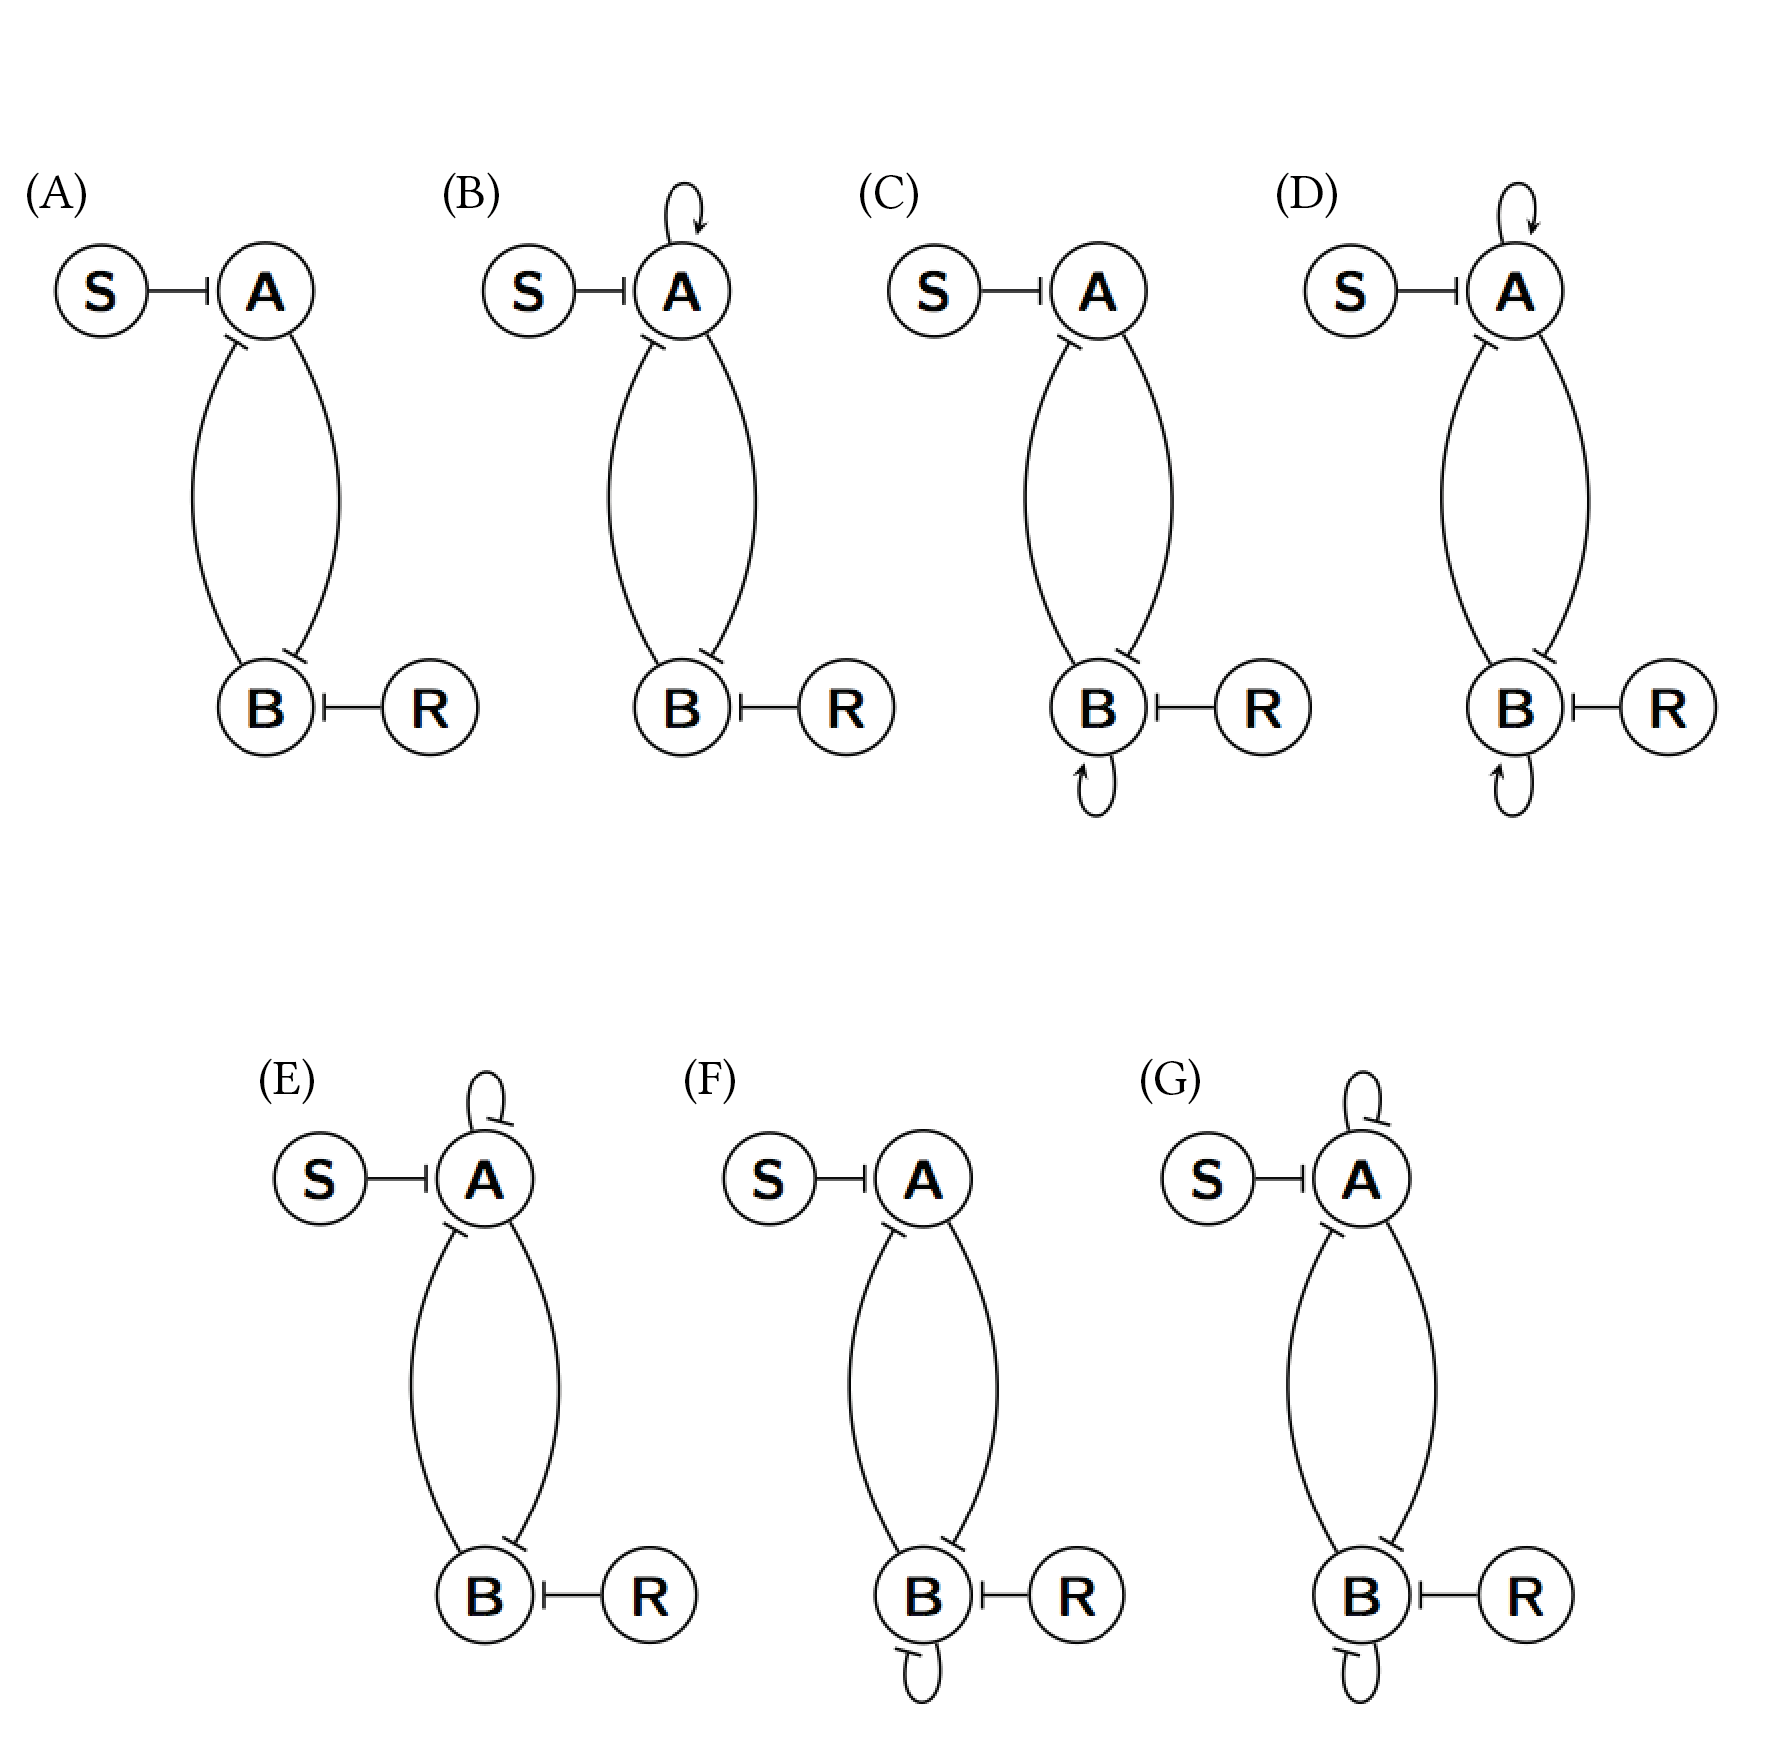
\includegraphics[width=\textwidth]{../../chapters/chapterABCSysBio/images/toggle_switch_designs.png}
\caption[Model designs considered for model selection.]{\label{fig:toggle_switch_designs}Toggle switch designs considered for model selection. 7 models were used: The simple toggle switch (A), the switches with positive autoregulation on either or both nodes (B, C, D) and the switches with negative autoregulation on either or both nodes (E, F, G)}
\end{center}
\end{figure*}
\clearpage

\subsubsection{Autoregulation switches phase space and bifurcation analysis}
\label{sec:models_bist_bif}
In order to use these models for model selection, it must first be determined whether they are capable of behaving like a switch. \acrshort{abc} \acrshort{smc} model selection is used to select models that can produce the same behaviour, over a greater range of parameter values. If a model is not capable of producing the desired behaviour for the prior range, then it will not be used for model selection.

I used the PyDSTool~\autocite{Clewley:2012kj} in order to determine whether each of the 7 switches is capable of bistable behaviour. The same analysis as Section~\ref{sec:bifurc} was used to identify the steady states of the systems and their stabilities. As shown in Figure~\ref{fig:Gard_pos}, both single and double positive autoregulation is consistent with bistable behaviour. Two stable states were found for both cases when $k$ = 2 and δ = 1. 


\begin{figure*}[htbp]
	\begin{center}
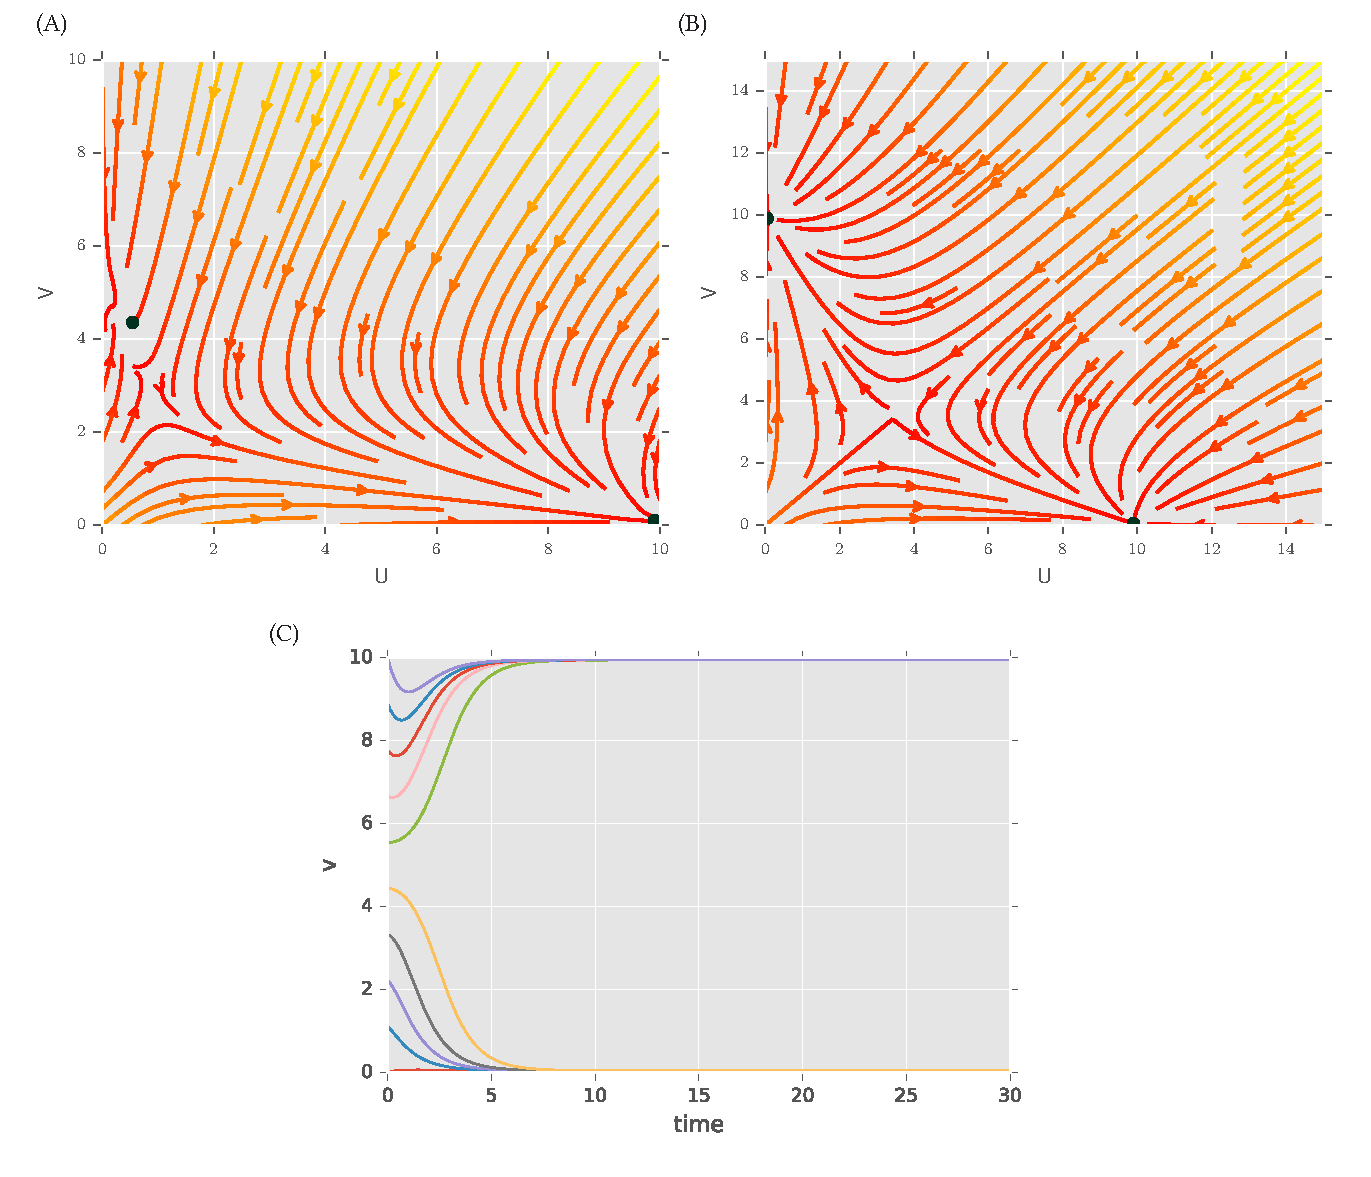
\includegraphics[scale=0.6]{../../chapters/chapterABCSysBio/images/gard_pos.pdf}
\caption[Phase plane analysis of the switch with positive autoregulation]{\label{fig:Gard_pos}Both single and positive autoregulation are consistent with bistable behaviour.  (A) Single positive autoregulation. Two stable steady states are found in the single positive autoregilation model at (u, v) = (9.89, 0.55) and (u, v) = (4.36, 0.1). (B) Double positive autoregulation. The model with double positive autoregulation has two stable steady states at (u, v) = (0.051, 9.89) and (u,v) = (9.89, 0.051).}
\end{center}
\end{figure*}


% A bifurcation analysis, when all other parameters are kept constant and only $k$ varied, shows that  even small values of $k$ destroy bistability. This is shown in Figure~\ref{fig:Gard_neg}C.

On the other hand, negative autoregulation was not consistent with bistable behaviour for the parameter values used here. The vector plot of the switch with single negative autoregulation show that there is one stable steady state when the levels of the unregulated protein are high and the levels of the negatively regulated protein low. The vector plot for the switch with double negative autoregulation shows one stable steady state when the levels of both proteins are low. A bifurcation plot of the switch with single positive autoregulation highlights this result; the switch is bistable for only very small amounts of $ka_1$, the parameter for negative autoregulation. This is shown in Figure~\ref{fig:Gard_neg}.

Negative autoregulation occurs when the protein binds to its own promoter and represses production. Therefore the protein levels rise to a lower level than what would be expected for an unregulated system~\autocite{Alon:2007}. In the case of the double negative autoregulation, the concentration levels of either protein would therefore not be sufficient to dominate over the other and create bistability. In the case of the single negative autoregulation, only the protein without autoregulation is able to reach sufficient levels to dominate the system, and thus the only steady state of the system is when the unregulated protein is high.


% (C) Bifurcation diagram of the single negative autoregulation switch, where all parameters remain constant and only $ku$ varied.
\begin{figure*}[htbp]
\centerfloat
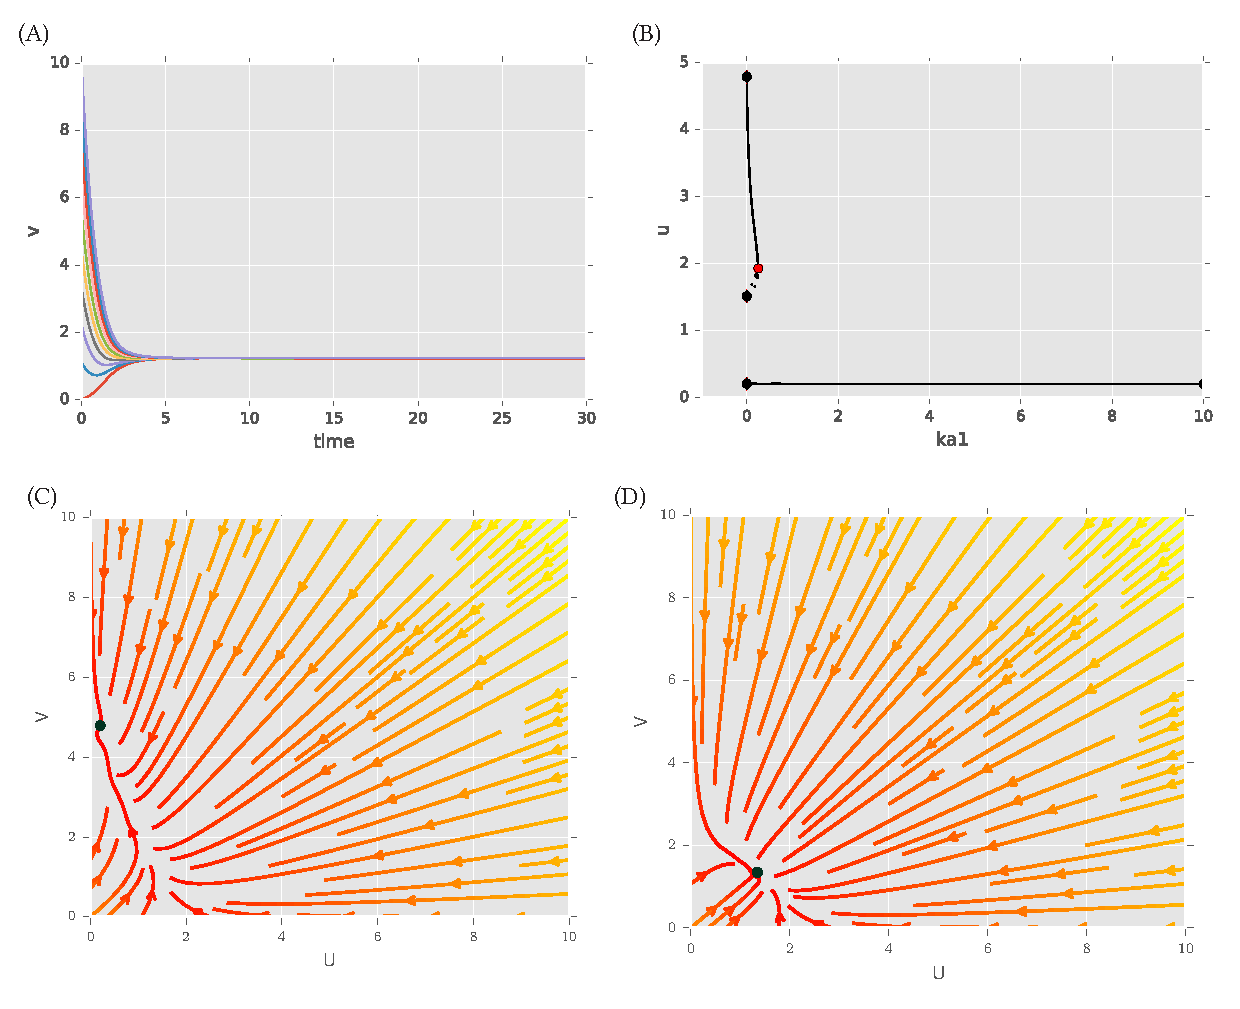
\includegraphics[scale=0.7]{../../chapters/chapterABCSysBio/images/gard_neg.pdf}
\caption[Phase plane and bifurcation analysis of the switch with negative autoregulation]{\label{fig:Gard_neg}(A) Time course of the single negative autoregulation switch, when $k_u$=2 with varying initial conditions. The system is monostable. (B) Bifurcation diagram with respect to parameter $ka_1$ of the switch with single negative autoregulation. The system is bistable only for very small amounts of $ka_1$. (C) One stable steady state is found for the single negative autoregulation switch when $k_u$ = 2 at u = 0.208 and v = 4.79. (C) The vector plot of the switch with double negative autoregulation has one steady state at u = 1.346 and v=1.346.}

\end{figure*}
\clearpage

The models shown here to be capable of bistable behaviour will be used in the following section for model selection, to determine whether the addition of positive feedback loops increases the robustness of the system to parameter fluctuations.

%the rational comparison of models under parameter uncertainty using Bayesian model selection, which automatically accounts for model complexity (number of parameters) and robustness to parameter uncertaint


\subsection{\acrshort{abc} for model selection}

In Section~\ref{sec:param_inf} I used ABC SMC to infer the parameters of a model that can produce the desired behaviour. In this Section I extend the analysis by asking which model, out of the 5 candidate models shown above, can best produce the desired behaviour. Bayesian model selection can be used to rank models according to their posterior distributions. 

ABC SMC model selection works by treating each model as another 'parameter'. ABC SMC then proceeds to approximate the posterior distribution over the joint space of all models~\autocite{Toni:2009tr}. The marginal posterior distribution (also known as model evidence) for each model ($m$) can then be used to rank all the models ($M$). 

\begin{align}
	p(m|D) = \frac{\textnormal{accepted particles from } m}{\textnormal{all accepted particles}}
\end{align}

ABC SMC model selection accounts for model complexity and parametric robustness in order to avoid the problem of overfitting. It automatically applies the rule of parsimony, or Occam's razor, which dictates the simplest model to account for the data is the best model~\autocite{Toni:2010}. This is done be penalising the addition of a parameter, corresponding to an increase in the volume of the prior,  if it does not result in a larger increase in the volume of the approximated posterior distribution~\autocite{Woods:2016eh}.  Bayesian model selection can be used to rank models according to how well they describe the data, or how likely they are to give rise to the data we wish to see in a system design setting.  


%Bayesian model selection is used to directly compare the competing designs using ABC-SysBio~\autocite{Liepe:2010eg}. This method enables the simultaneous inference of the kinetic parameters and the structure of the models in order to select the model producing the same behaviour over a greater parameter range. \acrshort{abc} \acrshort{smc} can be used for model selection by adding the model as a parameter to the selection process. The algorithm samples models as well as parameters at each iteration. When the last \textepsilon{} is reached, the algorithm will have concluded to a posterior distribution of parameters for each model, a subset of the prior distribution that can give the best rise to the data. The model that performs over a greater posterior parameter range is selected as the most robust~\autocite{Toni:2009tr}. The process is outlined in Figure~\ref{fig:abc_model_sel}.
    
%\begin{figure*}[htbp]
%	\begin{center}
%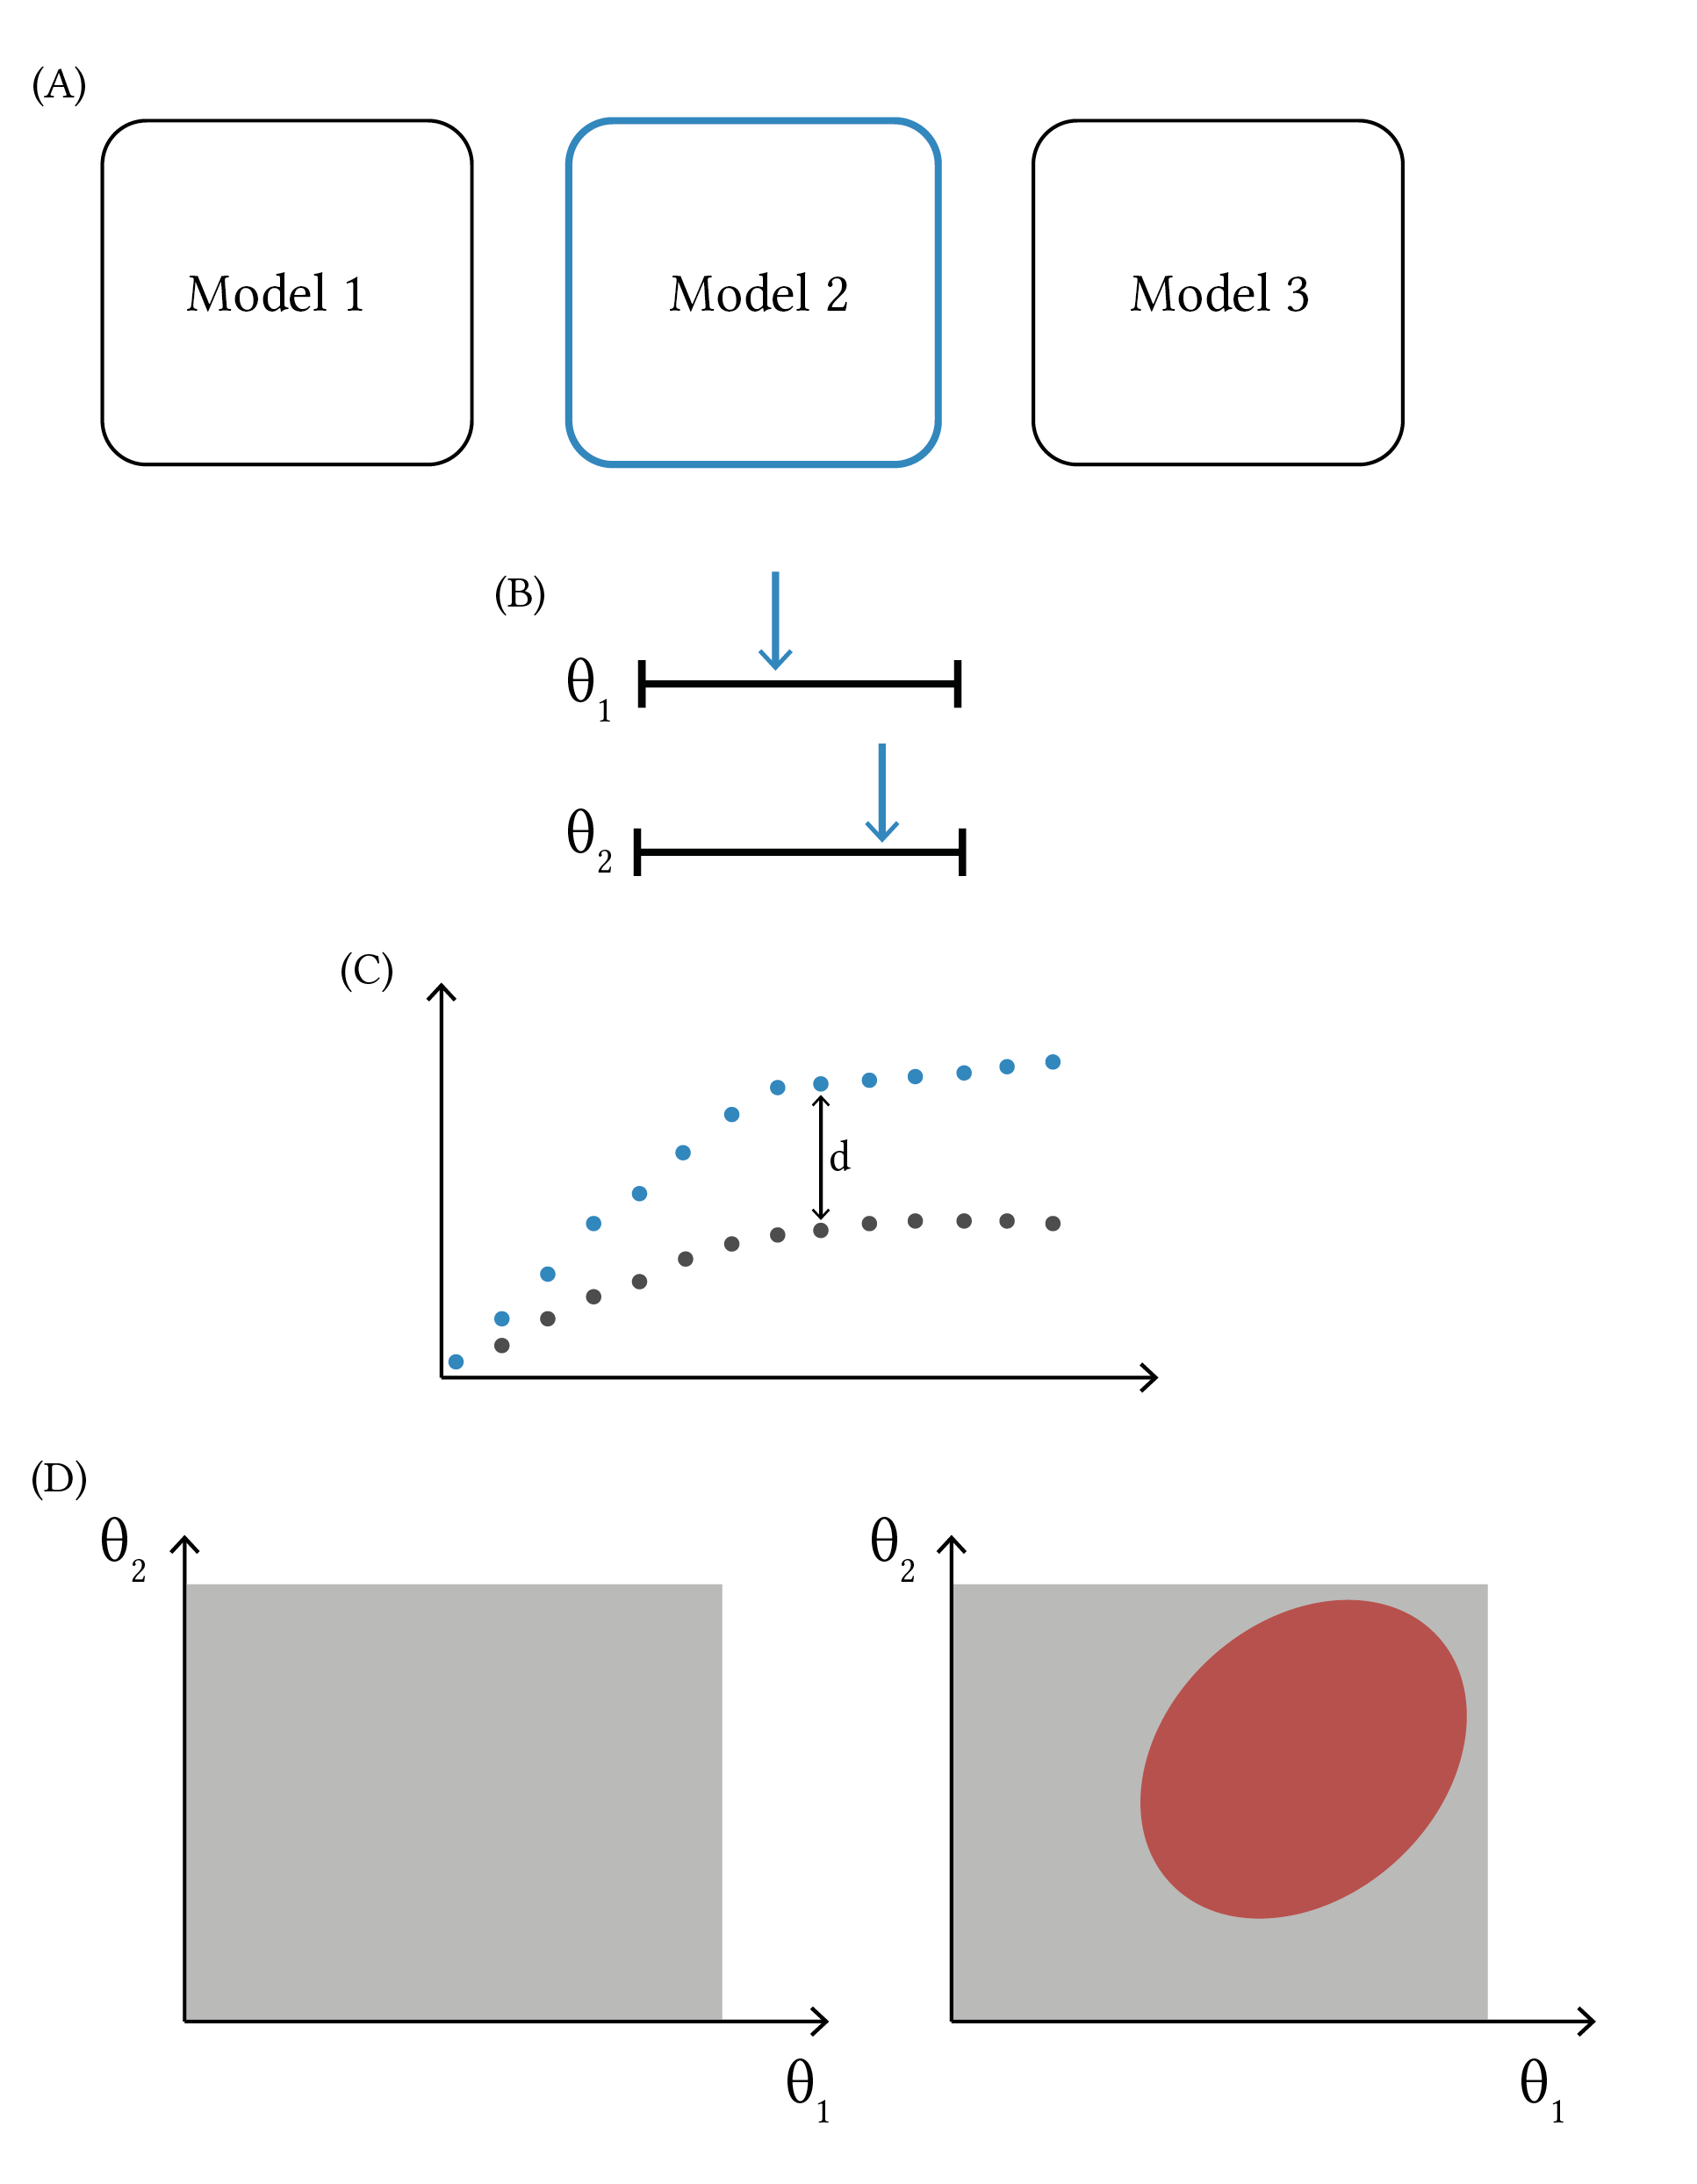
\includegraphics[scale=0.7]{../../chapters/chapterABCSysBio/images/model_selection.png}
%\caption[\acrshort{abc} \acrshort{smc} model selection]{\label{fig:abc_model_sel} \acrshort{abc} \acrshort{smc} model selection. (A) A model is sampled, and the (B) parameter values for that model are sampled. The system is simulated and the result compared to the desired behaviour. (C) If the distance between the two is smaller than the current accepted threshold, then the samples are retained. If not they are discarded. (D) This method can select the model that can produced the desired behaviour over a greater parameter range (red ellipse). }
%\end{center}
%\end{figure*}
%\clearpage


Here I apply ABC SMC model selection using the package ABC-SysBio~\autocite{Liepe:2010eg}. I study whether the addition of feedback loops to the standard toggle switch can increase its parametric robustness. The standard toggle switch was compared to switches with positive autoregulation in one or both nodes, which were shown to be capable of bistable behaviour in Section~\ref{sec:models_bist_bif}. The mass action models were used for model selection, in order to represent the system in a more realistic way. The equations shown in Table~\ref{tab:autoreg_equs} are added to the equations of the simple toggle switch used in Section~\ref{sec:param_inf}. Toggle switches with autoregulation on both nodes have both sets of equations added. The same design specifications as used in Section~\ref{sec:param_inf} were used.



\begin{table}[htbp]
\centering
\caption{Autoregulated switches additional equations}
\label{tab:autoreg_equs}
\begin{tabular}{@{}ll@{}}
\toprule
Equations                                                                              & Description             \\ \midrule
\multicolumn{2}{c}{ Positive autoregulation A}                                                                 \\\midrule
$\textrm{A2} + \textrm{gA} \stackrel{\textrm{aut\_1}}{\longrightarrow} \textrm{A2gA}$  & dimer self-association  \\
$\textrm{A2gA} \stackrel{\textrm{aut\_2}}{\longrightarrow} \textrm{A} + \textrm{A2gA}$ & self-induced expression \\
$\textrm{A2gA} \stackrel{\textrm{aut\_3}}{\longrightarrow} \textrm{A2}+ \textrm{gA}$   & dimer self-dissociation \\\midrule
\multicolumn{2}{c}{Positive autoregulation B}                                                                    \\\midrule
$\textrm{B2} + \textrm{gB} \stackrel{\textrm{aut\_1}}{\longrightarrow} \textrm{B2gB}$  & dimer self-association  \\
$\textrm{B2gB} \stackrel{\textrm{aut\_2}}{\longrightarrow} \textrm{B} + \textrm{B2gB}$ & self-induced expression \\
$\textrm{B2gB} \stackrel{\textrm{aut\_3}}{\longrightarrow} \textrm{B2}+ \textrm{gB}$   & dimer self-dissociation \\ \bottomrule
\end{tabular}
\end{table}
%Positive autoregulation on A:
%
%$$
%\begin{array}{cccc} 
%    \textrm{A2} + \textrm{gA} \stackrel{\textrm{aut\_1}}{\longrightarrow} \textrm{A2gA} \\
%    \textrm{A2gA} \stackrel{\textrm{aut\_2}}{\longrightarrow} \textrm{A} + \textrm{A2gA}\\
%    \textrm{A2gA} \stackrel{\textrm{aut\_3}}{\longrightarrow} \textrm{A2}+ \textrm{gA}  \\
%\end{array}
%$$
%
%Positive autoregulation on B:
%
%$$
%\begin{array}{cccc} 
%    \textrm{B2} + \textrm{gB} \stackrel{\textrm{aut\_1}}{\longrightarrow} \textrm{B2gB} \\
%    \textrm{B2gB} \stackrel{\textrm{aut\_2}}{\longrightarrow} \textrm{B} + \textrm{B2gB}\\
%    \textrm{B2gB} \stackrel{\textrm{aut\_3}}{\longrightarrow} \textrm{B2}+ \textrm{gB}  \\
%\end{array}
%$$

%Negative autoregulation on A:
%
%$$
%\begin{array}{cccc} 
%    \textrm{A2} + \textrm{gA} \stackrel{\textrm{aut\_1}}{\longrightarrow} \textrm{A2gA} \\
%    \textrm{A2gA} \stackrel{\textrm{aut\_2}}{\longrightarrow} \textrm{A2}+ \textrm{gA}  \\
%\end{array}
%$$
%
%Negative autoregulation on B:
%
%$$
%\begin{array}{cccc} 
%    \textrm{B2} + \textrm{gB} \stackrel{\textrm{aut\_1}}{\longrightarrow} \textrm{B2gB} \\
%    \textrm{B2gB} \stackrel{\textrm{aut\_2}}{\longrightarrow} \textrm{B2}+ \textrm{gB}  \\
%\end{array}
%$$

Given the models shown above and the parameter priors shown in Table~\ref{tab:model_selec_params}, ABC SMC model selection was carried out. The priors for model selection were set to wider that in the ones used during parameter inference of the simple switch in order to make them more flexible for the additional models. For all models initial conditions of the two genes, $gA$, $gB$ were set to 1, and species $A$ and $A2$ were set to 50 and 10 respectively, in order to set the starting conditions of the switch to $B2$ OFF. All other species initial conditions were set to 0. 

\begin{table}[htbp]
\centerfloat
\caption{The prior distributions used for model selection. The values indicate the lower and upper limits of a uniform distribution.}
\label{tab:model_selec_params}
\resizebox{1.3\textwidth}{!}{\begin{tabular}{ccccccccccccc}
\toprule
 \textbf{ge}     & \textbf{rep}     & \textbf{rep\_r}     & \textbf{dim}    & \textbf{dim\_r}     & \textbf{deg}  & \textbf{rep\_dim}    & \textbf{rep\_dim\_r} & \textbf{deg\_sr}  & \textbf{deg\_dim}   & \textbf{aut\_1} & \textbf{aut\_2} & \textbf{aut\_3} \\
  (min\textsuperscript{-1})&(μM min\textsuperscript{-1})&(min\textsuperscript{-1})&(μM min\textsuperscript{-1})&(min\textsuperscript{-1})&(min\textsuperscript{-1})&(μM min\textsuperscript{-1})&(min\textsuperscript{-1})&(min\textsuperscript{-1})&(min\textsuperscript{-1}) &(μM min\textsuperscript{-1})&(min\textsuperscript{-1})&(min\textsuperscript{-1})\\
1-10     & 1-10    & 0-5       & 1-10   & 0-5       & 1-5  & 0.05-0.1   & 0.01-0.1     & 0.01-0.1 & 0-1 & 0-10 & 0-2 & 0-10        \\ \bottomrule
\end{tabular}}
\end{table}


\begin{figure*}[htbp]
	\centerfloat
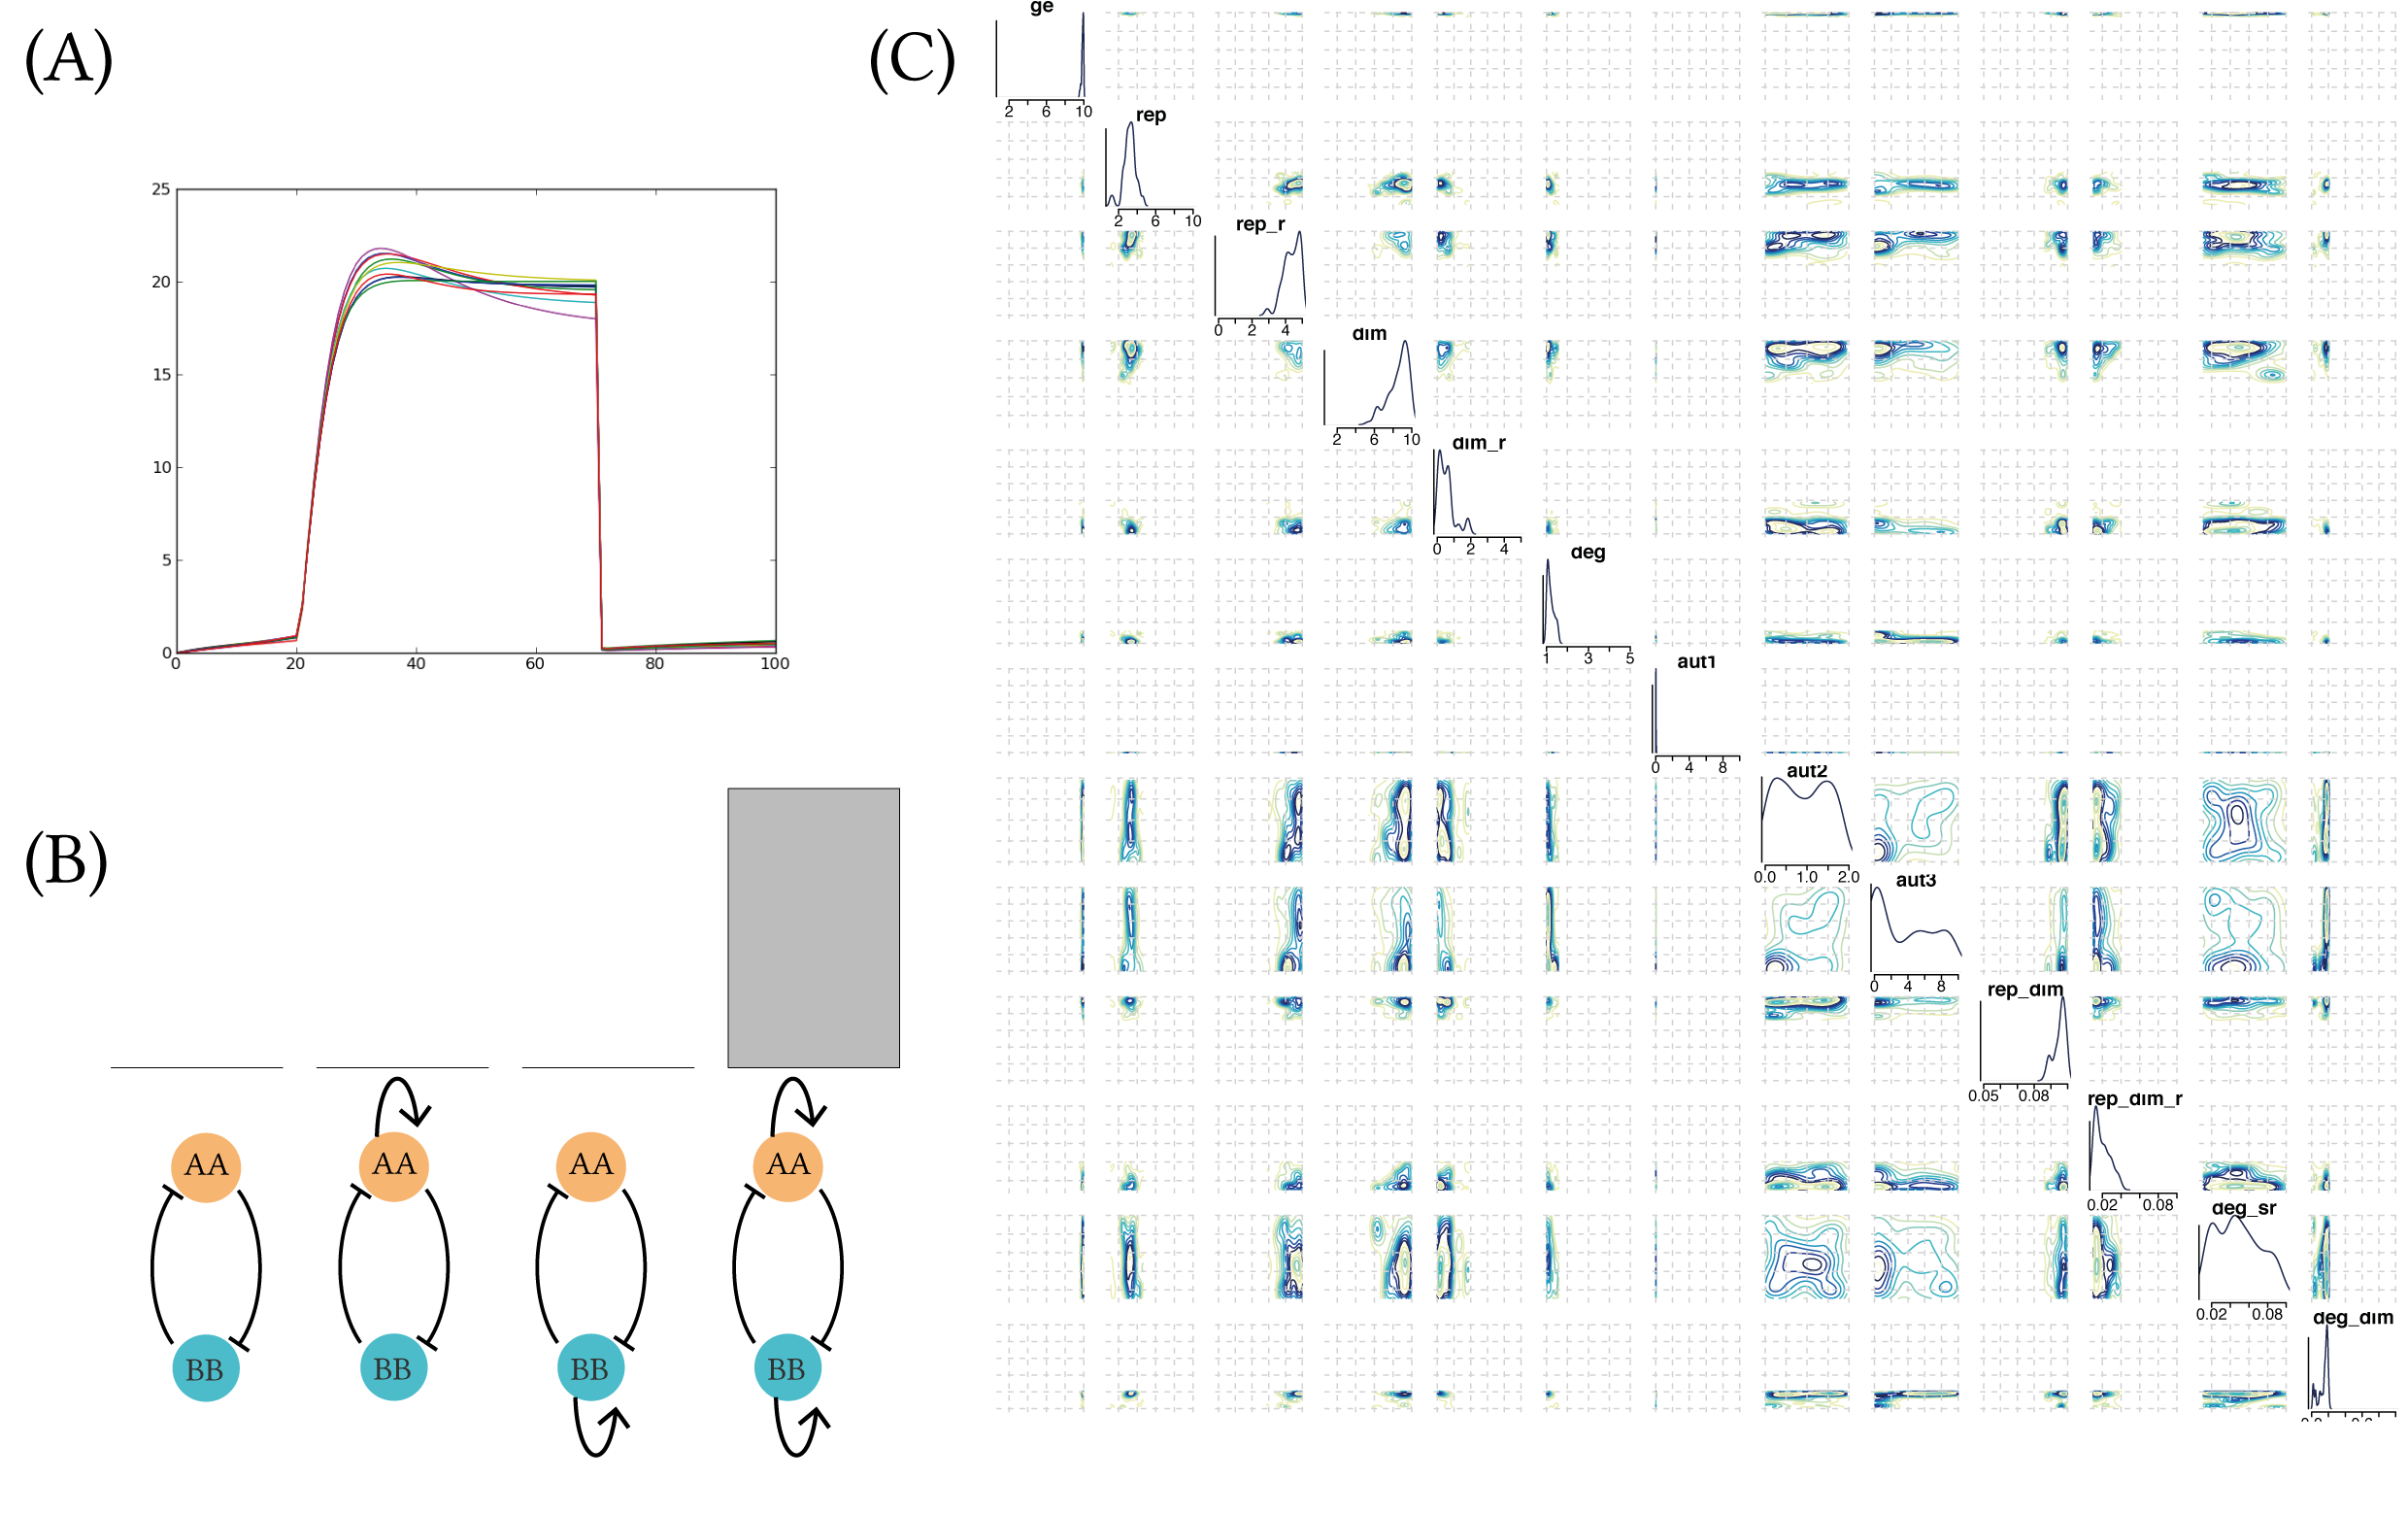
\includegraphics[scale=0.75]{../../chapters/chapterABCSysBio/images/model_sel_res-01.png}
\caption[ABC model selection resulting posterior distribution]{\label{fig:model_sel_res}: (A) The simulated time course of the last population of the switch with double positive autoregulation. (B) The toggle switch with positive autoregulation on both nodes was found to be the most robust to parameter fluctuations. Three repeats of the model selection were carried out, and the median values are shown here. Upper and lower quartile error bars are included but are too small to be visible. (C) The posterior distribution of the toggle switch with positive autoregulation on A and B.}


\end{figure*}
\clearpage
The results are shown in Figure~\ref{fig:model_sel_res}. The toggle switch with positive autoregulation on both nodes was found to be the most robust model. This indicates that although all the models considered are capable of behaving like a switch, the model with double positive autoregulation could do that over a greater parameter range.  



\section{Discussion}

Here I developed a more realistic model for the genetic toggle switch, using mass action which does not use the \acrshort{qssa}. In Chapter~\ref{ch:SF} I explore this model further and show that the \acrshort{qssa} cannot always be justified. I showed that this model is capable of bistable behaviour, within a given parameter range. I further studied this by using \acrshort{abc} \acrshort{smc} parameter inference to fit the toggle switch to a switching behaviour of choice. The parameter inference revealed the range of parameter values that can produce the behaviour of choice. These parameter values can be used to design a synthetic toggle switch that will behave in the specified manner. 

Further, I showed that negative autoregulation is not consistent with bistable behaviour for the parameter values examined here. Adding small levels of single negative autoregulation to the system caused it to revert to monostability. The only steady state was when the unregulated protein was high and the negatively regulated protein was low. This makes sense, as the negatively regulated protein cannot reach high enough levels to repress the other protein and dominate the system, whereas the unregulated protein is free to reach a higher steady state. In the case of double negative autoregulation, neither protein is free to reach sufficient levels to dominate the other, and the only steady state was when the levels of both proteins are low. This indicates that the system reaches a deadlock situation where both proteins are repressed and cannot reach a higher steady state. The models used here are deterministic and simplified down to two equations. Stochastic dynamics where noise is added to the system or a more complex model could be capable of overcoming this deadlock situation. More specifically, if transcriptional or translational bursting is included, the protein that receives the first boost can dominate the system on time and escape the deadlock situation~\autocite{Strasser:2012kt}.


Finally, I showed that the addition of positive feedback loops make the genetic toggle switch more robust to parameter fluctuations. This means that the model was capable of producing the desired behaviour over a greater parameter range. This indicates that small fluctuations in parameters in the cellular environment will not affect the system's ability to be bistable, and thus makes it more suitable for use in synthetic biological applications where a very constrained parameter set can be too restrictive. This makes it a better candidate for building new synthetic devices based on the toggle switch design.
 

%The first computational approach for the tuning of robust synthetic networks was that of Batt \textit{et al}, ~\cite{Batt:2007jl} where they examined the problem of finding a subset of the parameter set for which a given property was satisfied for all the parameters.  An evolutionary algorithm has also been used to solve the robust design problem by evolving the parameters of the system in order to make it more robust to cellular disturbances by Chen \textit{et al} ~\cite{Chen:2011hj}. The added value of the methodology presented here is that the network structure in addition to the network parameters are adjusted to select a network that can robustly create the desired behaviour.


The volume of the posterior distribution of even the most robust switch out of the ones examined here was still not large. This means that the behaviour of choice is still constrained, even after the addition of the positive feedback loops. A caveat of the analysis used here that has to be considered is that the parameter space is not searched for simply combinations that can produce a bistable switch. The behaviour that is required is very specific, and it is probable that the plethora of constraints put to the system result in the discard of parameter combinations that create a bistable switch. Firstly, a specific steady state level is required, for both the ON and OFF stages. When the switch is OFF, the protein levels must be as close to zero as possible, and when the switch is ON, the protein levels are required to approach 20μM. This requirement will discard any switches that have a higher or lower ON state, or a slightly higher OFF state. Additionally, the design specifications used here dictate that the time to reach steady state has to be quick. There is not much transition time allowed between the ON and OFF states, and the protein is required to reach steady state within a few time points. Here, model time was taken to represent minutes, thus a time point in the simulation represents on minute. This dictates that the switch has to occur very fast. This results in the exclusion of systems that reach steady state slower, but still act as a bistable switch. Therefore, the switches examined here, follow a very constrained behaviour. In the next Chapter I develop a method that is more flexible in the type of switches it can analyze.     

It is important to discuss the assumptions made in the models presented in this Chapter. As was discussed in Chapter~\ref{ch:backg}, the assumptions made about the underlying model can affect the behaviour observed in the model. Firstly, the numerous steps involved in transcription and translation have been condensed into one 'gene expression' step.  This simplifies the model by reducing the number of parameters an reactions included, and it has been shown that it does not affect the stability of the switch~\autocite{Warren:2005kea}. The other assumption being made here is that repression is cooperative. This means that a transcription factor dimer has to bind to the promoter region to repress it successfully. This has been shown to be critical for a bistable switch~\autocite{Gardner:2000vha, Warren:2005kea, Warren:2004baa, Cherry:2000wi}, as discussed in Chapter~\ref{ch:backg}.~\textcite{Lipshtat:2006wb} found that a switch can be exhibit bistability without cooperativity, only if stochasticity is taken into account. Since the switch models were simulated using deterministic dynamics here, the assumption of cooperativity was necessary to make it bistable. Finally, the models used here correspond to a general switch, i.e. a switch where both repressors A2 and B2 are free to bind to the promoters simultaneously. This is in contrast to the exclusive switch, where the two promoters are assumed to overlap and the two proteins cannot bind at the same time~\autocite{Loinger:2007vma}. The exclusive switch can be found in natural systems~\autocite{lambda_sw} and has been shown that the exclusive switch is more robust than the general switch~\autocite{Loinger:2007vma, Barnes:2011hh}. Nevertheless, here I model a synthetic genetic switch, like the one build by~\textcite{Gardner:2000vha}, which consists of two separate promoters, making the general switch model more appropriate. 


%Further analysis is thus needed to determine what these combinations are. A sensitivity analysis of the model will be carried out in order to determine which parameters affect bistability and to which parameters is the system robust. The parameter scan will also be incorporated into the ABC SMC methodology, in order to identify the parameter values required for bistability more efficiently.             

%In this work it was shown that a range of stability profiles are achievable by the standard toggle switch. The patterns of the parameter values required for each are beginning to emerge. Further work is required in order to get a definitive answer for the stability characteristics of the toggle switch given this modelling approach.


	
%Chen \textit{et al} ~\cite{Chen:2009ea} used the fuzzy  dynamic game method to solve the minimax regulation design problem of synthetic genetic networks. In that method the worst case effect of all disturbances is minimised for a given network.

\section{Summary}

In this chapter I studied the~\textcite{Gardner:2000vha} toggle switch and showed that it is bistable. I further studied the genetic toggle switch model using mass action. I identified the parameter ranges that produce a bistable behaviour and could be used as prior distributions for parameter inference. Further, I studied the effect of adding feedback loops has on the robustness of the genetic toggle switch. I found that the switch with double positive autoregulation is the most robust to parameter fluctuations. In the next chapter I address some of the shortcomings of the method used here by developing a new algorithm, StabiliyFinder. 


